% ============================================================================
% DIP-SMC-PSO Comprehensive Project Presentation
% ============================================================================
% A complete technical overview covering all aspects of the project
% from foundational theory to production infrastructure
%
% Target: 350+ slides for PhD defense / academic conference presentation
% ============================================================================

% ============================================================================
% Beamer Configuration for DIP-SMC-PSO Comprehensive Presentation
% ============================================================================
% This file contains all preamble settings, packages, and custom commands
% shared across the main presentation and speaker scripts.
% ============================================================================

% Document class for Beamer presentations
\documentclass[aspectratio=169,10pt]{beamer}

% ============================================================================
% Theme and Appearance
% ============================================================================
\usetheme{Madrid}
\usecolortheme{default}
\setbeamertemplate{navigation symbols}{}
\setbeamertemplate{footline}[frame number]
\setbeamertemplate{caption}[numbered]

% ============================================================================
% Essential Packages
% ============================================================================
\usepackage[utf8]{inputenc}
\usepackage[T1]{fontenc}
\usepackage{lmodern}
\usepackage{amsmath,amssymb,amsfonts}
\usepackage{mathtools}
\usepackage{graphicx}
\usepackage{booktabs}
\usepackage{multirow}
\usepackage{array}
\usepackage{xcolor}
\usepackage{tikz}
\usetikzlibrary{shapes,arrows,positioning,calc,decorations.pathreplacing}
\usepackage{pgfplots}
\pgfplotsset{compat=1.18}
\usepackage{algorithm}
\usepackage{algpseudocode}
\usepackage{listings}
\usepackage{hyperref}

% ============================================================================
% Code Listings Configuration (Python)
% ============================================================================
\lstset{
    language=Python,
    basicstyle=\ttfamily\footnotesize,
    keywordstyle=\color{blue}\bfseries,
    commentstyle=\color{gray}\itshape,
    stringstyle=\color{red},
    numbers=left,
    numberstyle=\tiny\color{gray},
    stepnumber=1,
    numbersep=5pt,
    backgroundcolor=\color{white},
    showspaces=false,
    showstringspaces=false,
    showtabs=false,
    frame=single,
    tabsize=4,
    captionpos=b,
    breaklines=true,
    breakatwhitespace=false,
    escapeinside={\%*}{*)},
    morekeywords={self,True,False,None},
}

% ============================================================================
% Custom Colors
% ============================================================================
\definecolor{dipblue}{RGB}{0,102,204}
\definecolor{dipgreen}{RGB}{0,153,76}
\definecolor{dipred}{RGB}{204,0,0}
\definecolor{diporange}{RGB}{255,128,0}
\definecolor{dipgray}{RGB}{128,128,128}

% ============================================================================
% Custom Commands - Mathematical Notation
% ============================================================================

% State vectors
\newcommand{\statevec}{\mathbf{x}}
\newcommand{\controlvec}{\mathbf{u}}
\newcommand{\outputvec}{\mathbf{y}}

% Common operators
\newcommand{\der}[2]{\frac{d#1}{d#2}}
\newcommand{\pder}[2]{\frac{\partial #1}{\partial #2}}
\newcommand{\norm}[1]{\left\|#1\right\|}
\newcommand{\abs}[1]{\left|#1\right|}
\newcommand{\sign}{\text{sign}}
\newcommand{\sat}{\text{sat}}

% Sliding surface
\newcommand{\slidingsurf}{s}
\newcommand{\slidingsurfvec}{\mathbf{s}}

% Lyapunov function
\newcommand{\lyap}{V}

% Common matrices
\newcommand{\massmatrix}{\mathbf{M}}
\newcommand{\coriolismatrix}{\mathbf{C}}
\newcommand{\gravitymatrix}{\mathbf{G}}
\newcommand{\inputmatrix}{\mathbf{Q}}

% ============================================================================
% Custom Commands - Annotations
% ============================================================================
\newcommand{\highlight}[1]{\textcolor{dipblue}{\textbf{#1}}}
\newcommand{\important}[1]{\textcolor{dipred}{\textbf{#1}}}
\newcommand{\success}[1]{\textcolor{dipgreen}{\textbf{#1}}}
\newcommand{\warning}[1]{\textcolor{diporange}{\textbf{#1}}}

% Status indicators
\newcommand{\statusok}{\textcolor{dipgreen}{[OK]}}
\newcommand{\statuserror}{\textcolor{dipred}{[ERROR]}}
\newcommand{\statuswarning}{\textcolor{diporange}{[WARNING]}}
\newcommand{\statusinfo}{\textcolor{dipblue}{[INFO]}}

% ============================================================================
% Custom Commands - Abbreviations
% ============================================================================
\newcommand{\dip}{DIP}
\newcommand{\smc}{SMC}
\newcommand{\pso}{PSO}
\newcommand{\sta}{STA}
\newcommand{\mpc}{MPC}
\newcommand{\hil}{HIL}
\newcommand{\qa}{QA}

% ============================================================================
% Bibliography Setup
% ============================================================================
\usepackage[style=numeric,sorting=none,backend=biber]{biblatex}
\addbibresource{references.bib}

% ============================================================================
% Title Information
% ============================================================================
\title[DIP-SMC-PSO: Comprehensive Overview]{%
    Double-Inverted Pendulum Sliding Mode Control \\
    with PSO Optimization: \\
    A Comprehensive Technical Overview%
}

\author{%
    Sadegh Naderi%
}

\institute{%
    GitHub: https://github.com/theSadeQ/dip-smc-pso.git
}

\date{\today}

% ============================================================================
% Hyperref Configuration
% ============================================================================
\hypersetup{
    colorlinks=true,
    linkcolor=dipblue,
    urlcolor=dipblue,
    citecolor=dipgreen,
    pdfauthor={Sadegh Naderi},
    pdftitle={DIP-SMC-PSO Comprehensive Presentation},
    pdfsubject={Control Systems, Sliding Mode Control, Particle Swarm Optimization},
    pdfkeywords={Double Inverted Pendulum, Sliding Mode Control, PSO, Control Theory}
}

% ============================================================================
% Custom Blocks
% ============================================================================
\setbeamercolor{block title}{bg=dipblue,fg=white}
\setbeamercolor{block body}{bg=dipblue!10,fg=black}

\setbeamercolor{block title example}{bg=dipgreen,fg=white}
\setbeamercolor{block body example}{bg=dipgreen!10,fg=black}

\setbeamercolor{block title alerted}{bg=dipred,fg=white}
\setbeamercolor{block body alerted}{bg=dipred!10,fg=black}

% ============================================================================
% End of Configuration
% ============================================================================


\begin{document}

% ============================================================================
% TITLE SLIDE
% ============================================================================
\begin{frame}
    \titlepage
\end{frame}

% ============================================================================
% TABLE OF CONTENTS
% ============================================================================
\begin{frame}{Presentation Overview}
    \tableofcontents
\end{frame}

% ============================================================================
% PART I: FOUNDATIONS
% ============================================================================
\part{Foundations}
\frame{\partpage}

% ============================================================================
% SECTION 1: PROJECT OVERVIEW & INTRODUCTION
% ============================================================================
\section{Project Overview \& Introduction}

\begin{frame}{What is DIP-SMC-PSO?}
    \begin{columns}
        \begin{column}{0.5\textwidth}
            \textbf{System Description:}
            \begin{itemize}
                \item \highlight{Double-Inverted Pendulum} (DIP)
                \item Two poles stacked on a moving cart
                \item Highly unstable, nonlinear dynamics
                \item Classic control theory benchmark
            \end{itemize}

            \vspace{0.5cm}

            \textbf{Control Approach:}
            \begin{itemize}
                \item \highlight{Sliding Mode Control} (SMC)
                \item Seven controller variants
                \item \highlight{PSO Optimization} for gain tuning
                \item Comprehensive Python framework
            \end{itemize}
        \end{column}

        \begin{column}{0.5\textwidth}
            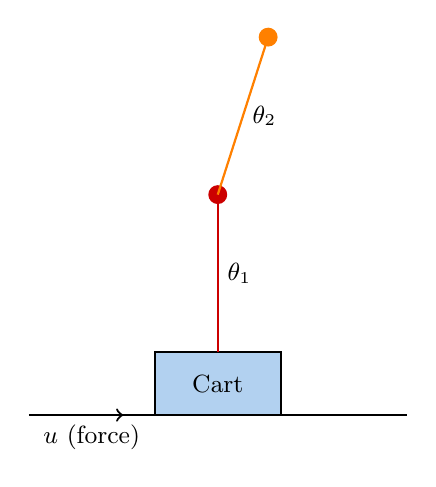
\begin{tikzpicture}[scale=0.8]
                % Cart
                \draw[fill=dipblue!30, thick] (-1,-0.5) rectangle (1,0.5);
                \node at (0,0) {\small Cart};

                % First pole
                \draw[thick, dipred] (0,0.5) -- (0,3);
                \fill[dipred] (0,3) circle (0.15);
                \node[right] at (0,1.75) {\small $\theta_1$};

                % Second pole
                \draw[thick, diporange] (0,3) -- (0.8,5.5);
                \fill[diporange] (0.8,5.5) circle (0.15);
                \node[right] at (0.4,4.25) {\small $\theta_2$};

                % Ground
                \draw[thick] (-3,-0.5) -- (3,-0.5);
                \draw[thick, ->] (-2.5,-0.5) -- (-1.5,-0.5);
                \node[below] at (-2,-0.5) {\small $u$ (force)};
            \end{tikzpicture}
        \end{column}
    \end{columns}
\end{frame}

\begin{frame}{Real-World Applications}
    \begin{block}{Why Study Inverted Pendulums?}
        Fundamental dynamics appear in numerous engineering systems
    \end{block}

    \vspace{0.3cm}

    \begin{columns}
        \begin{column}{0.5\textwidth}
            \textbf{Robotics:}
            \begin{itemize}
                \item Bipedal walking robots
                \item Humanoid balance control
                \item Segway-type vehicles
                \item Quadruped locomotion
            \end{itemize}

            \vspace{0.3cm}

            \textbf{Aerospace:}
            \begin{itemize}
                \item Rocket landing (SpaceX Falcon 9)
                \item Satellite attitude control
                \item Launch vehicle stabilization
            \end{itemize}
        \end{column}

        \begin{column}{0.5\textwidth}
            \textbf{Industrial:}
            \begin{itemize}
                \item Crane anti-sway systems
                \item Tower crane load stabilization
                \item Bridge construction equipment
            \end{itemize}

            \vspace{0.3cm}

            \textbf{Drones \& UAVs:}
            \begin{itemize}
                \item Quadcopter stabilization
                \item Tilt-rotor aircraft
                \item VTOL transitions
            \end{itemize}
        \end{column}
    \end{columns}
\end{frame}

\begin{frame}{Project Scope}
    \textbf{Comprehensive Python Framework for:}

    \vspace{0.3cm}

    \begin{enumerate}
        \item \highlight{Simulation} -- High-fidelity nonlinear dynamics, multiple integrators
        \item \highlight{Control} -- Seven SMC variants (Classical, STA, Adaptive, Hybrid, Swing-up, MPC)
        \item \highlight{Optimization} -- PSO-based automatic gain tuning
        \item \highlight{Analysis} -- Performance metrics, statistical validation, Monte Carlo
        \item \highlight{Visualization} -- Real-time animations, publication-ready plots
        \item \highlight{Testing} -- 668 tests, 100\% pass rate, production-grade quality
        \item \highlight{Documentation} -- 985 files, 12,500+ lines, complete learning paths
        \item \highlight{HIL Support} -- Hardware-in-the-loop for physical experiments
    \end{enumerate}

    \vspace{0.3cm}

    \begin{alertblock}{Current Status}
        \success{Phase 5 COMPLETE} -- Research-ready, LT-7 paper SUBMISSION-READY
    \end{alertblock}
\end{frame}

\begin{frame}{Project Scale \& Maturity}
    \begin{columns}
        \begin{column}{0.5\textwidth}
            \textbf{Codebase Metrics:}
            \begin{itemize}
                \item \highlight{328 Python files} (production)
                \item \highlight{668 tests} created (100\% pass)
                \item \highlight{2.86\% coverage} baseline (accurate)
                \item 100\% in 10 critical modules
                \item Thread-safe validated
            \end{itemize}

            \vspace{0.3cm}

            \textbf{Documentation:}
            \begin{itemize}
                \item \highlight{985 total files}
                \item 814 in docs/, 171 in .ai\_workspace/
                \item 12,500+ lines professional docs
                \item 11 navigation systems
                \item 43 category indexes
            \end{itemize}
        \end{column}

        \begin{column}{0.5\textwidth}
            \textbf{Research Outputs:}
            \begin{itemize}
                \item \highlight{11/11 research tasks} complete
                \item LT-7 paper SUBMISSION-READY
                \item 14 publication-ready figures
                \item Lyapunov proofs for 7 controllers
                \item Comprehensive benchmarks
            \end{itemize}

            \vspace{0.3cm}

            \textbf{Quality Metrics:}
            \begin{itemize}
                \item Production readiness: 63.3/100
                \item Memory management: 88/100 \statusok
                \item Thread safety: 100\% \statusok
                \item Documentation: 100/100 \statusok
            \end{itemize}
        \end{column}
    \end{columns}
\end{frame}

\begin{frame}{Project Timeline}
    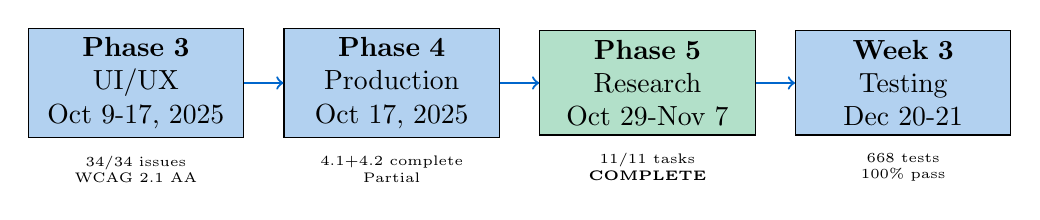
\begin{tikzpicture}[
        phase/.style={rectangle, draw, fill=dipblue!30, text width=2.5cm, align=center, minimum height=1cm},
        arrow/.style={->, thick, dipblue}
    ]
        % Phase 3
        \node[phase] (p3) at (0,0) {\textbf{Phase 3} \\ UI/UX \\ Oct 9-17, 2025};
        \node[below=0.1cm of p3, text width=2.5cm, align=center, font=\tiny] {34/34 issues \\ WCAG 2.1 AA};

        % Phase 4
        \node[phase, right=0.5cm of p3] (p4) {\textbf{Phase 4} \\ Production \\ Oct 17, 2025};
        \node[below=0.1cm of p4, text width=2.5cm, align=center, font=\tiny] {4.1+4.2 complete \\ Partial};

        % Phase 5
        \node[phase, fill=dipgreen!30, right=0.5cm of p4] (p5) {\textbf{Phase 5} \\ Research \\ Oct 29-Nov 7};
        \node[below=0.1cm of p5, text width=2.5cm, align=center, font=\tiny] {11/11 tasks \\ \textbf{COMPLETE}};

        % Week 3 Coverage
        \node[phase, right=0.5cm of p5] (wk3) {\textbf{Week 3} \\ Testing \\ Dec 20-21};
        \node[below=0.1cm of wk3, text width=2.5cm, align=center, font=\tiny] {668 tests \\ 100\% pass};

        % Arrows
        \draw[arrow] (p3) -- (p4);
        \draw[arrow] (p4) -- (p5);
        \draw[arrow] (p5) -- (wk3);
    \end{tikzpicture}

    \vspace{0.5cm}

    \begin{block}{Phase 5 Research Roadmap (72 hours over 8 weeks)}
        \begin{itemize}
            \item \success{Week 1 (8h):} Benchmarks, chattering metrics, visualization
            \item \success{Weeks 2-4 (18h):} Comprehensive benchmark, boundary layer optimization
            \item \success{Months 2-3 (46h):} Lyapunov proofs, model uncertainty, research paper
        \end{itemize}
    \end{block}
\end{frame}

\begin{frame}{Key Achievements}
    \begin{exampleblock}{Research Contributions}
        \begin{itemize}
            \item \textbf{Seven SMC Controllers} -- Classical, STA, Adaptive, Hybrid, Swing-up, MPC + Factory
            \item \textbf{Lyapunov Stability Analysis} -- Formal proofs for all 7 controllers (~1,000 lines)
            \item \textbf{Comprehensive Benchmarks} -- 100 Monte Carlo runs × 7 controllers
            \item \textbf{Robust PSO Validation} -- MT-7 bonus task, integrated in paper
            \item \textbf{Model Uncertainty Analysis} -- ±10\%, ±20\% parameter variations (LT-6)
            \item \textbf{Submission-Ready Paper} -- LT-7 v2.1, 14 figures, IEEE/IFAC format
        \end{itemize}
    \end{exampleblock}

    \begin{exampleblock}{Engineering Contributions}
        \begin{itemize}
            \item \textbf{Production-Grade Architecture} -- Thread-safe, memory-bounded, validated
            \item \textbf{Automated Recovery System} -- 30-second context restoration after token limits
            \item \textbf{Educational Materials} -- Beginner roadmap (125-150 hrs), 44-episode podcast series
            \item \textbf{Documentation Infrastructure} -- 985 files, 11 navigation systems, Sphinx integration
        \end{itemize}
    \end{exampleblock}
\end{frame}

\begin{frame}{Technology Stack}
    \begin{columns}
        \begin{column}{0.5\textwidth}
            \textbf{Core Libraries:}
            \begin{itemize}
                \item \texttt{Python 3.9+}
                \item \texttt{NumPy} -- Numerical computing
                \item \texttt{SciPy} -- Scientific algorithms
                \item \texttt{Matplotlib} -- Visualization
                \item \texttt{Numba} -- JIT compilation
            \end{itemize}

            \vspace{0.3cm}

            \textbf{Optimization:}
            \begin{itemize}
                \item \texttt{PySwarms} -- PSO primary
                \item \texttt{Optuna} -- Hyperparameter tuning
                \item Custom PSO implementation
            \end{itemize}
        \end{column}

        \begin{column}{0.5\textwidth}
            \textbf{Testing \& QA:}
            \begin{itemize}
                \item \texttt{pytest} -- Test framework
                \item \texttt{pytest-benchmark} -- Performance
                \item \texttt{Hypothesis} -- Property-based
                \item \texttt{Playwright} -- Browser automation
            \end{itemize}

            \vspace{0.3cm}

            \textbf{Configuration:}
            \begin{itemize}
                \item \texttt{Pydantic} -- Validation
                \item \texttt{YAML} -- Config format
            \end{itemize}

            \vspace{0.3cm}

            \textbf{UI:}
            \begin{itemize}
                \item \texttt{Streamlit} -- Web interface
            \end{itemize}
        \end{column}
    \end{columns}
\end{frame}

\begin{frame}{Repository \& Open Source}
    \begin{block}{GitHub Repository}
        \centering
        \url{https://github.com/theSadeQ/dip-smc-pso.git}
    \end{block}

    \vspace{0.3cm}

    \textbf{Key Statistics:}
    \begin{itemize}
        \item \highlight{Main branch deployment} strategy
        \item \highlight{Automated state tracking} via Git hooks
        \item \highlight{30-second recovery} after token limits/interruptions
        \item \highlight{Multi-account support} for seamless collaboration
    \end{itemize}

    \vspace{0.3cm}

    \textbf{License \& Attribution:}
    \begin{itemize}
        \item \highlight{39 academic citations} for control theory
        \item \highlight{30+ software dependencies} with proper attribution
        \item \highlight{100\% license compliance}
        \item Complete BibTeX database for publications
    \end{itemize}
\end{frame}

% ============================================================================
% SECTION 2: CONTROL THEORY FOUNDATIONS
% ============================================================================
\section{Control Theory Foundations}

\begin{frame}{Seven Controller Types: Overview}
    \begin{enumerate}
        \item \highlight{Classical SMC} -- Boundary layer for chattering reduction
        \begin{itemize}
            \item Simplest implementation, robust to uncertainties
            \item \texttt{src/controllers/classical\_smc.py}
        \end{itemize}

        \item \highlight{Super-Twisting Algorithm (STA)} -- Continuous higher-order SMC
        \begin{itemize}
            \item Second-order sliding mode, finite-time convergence
            \item \texttt{src/controllers/sta\_smc.py}
        \end{itemize}

        \item \highlight{Adaptive SMC} -- Online parameter estimation
        \begin{itemize}
            \item Adapts to unknown system parameters
            \item \texttt{src/controllers/adaptive\_smc.py}
        \end{itemize}

        \item \highlight{Hybrid Adaptive STA-SMC} -- Combines adaptive + super-twisting
        \begin{itemize}
            \item Best of both approaches
            \item \texttt{src/controllers/hybrid\_adaptive\_sta\_smc.py}
        \end{itemize}
    \end{enumerate}
\end{frame}

\begin{frame}{Seven Controller Types: Advanced \& Experimental}
    \begin{enumerate}
        \setcounter{enumi}{4}
        \item \highlight{Swing-Up SMC} -- Large-angle stabilization
        \begin{itemize}
            \item Energy-based swing-up + SMC balance
            \item \texttt{src/controllers/swing\_up\_smc.py}
        \end{itemize}

        \item \highlight{Model Predictive Control (MPC)} -- Experimental optimization-based
        \begin{itemize}
            \item Predicts future states, optimizes control sequence
            \item \texttt{src/controllers/mpc.py}
        \end{itemize}

        \item \highlight{Factory Pattern} -- Thread-safe controller registry
        \begin{itemize}
            \item Unified interface for all controllers
            \item \texttt{src/controllers/factory.py}
        \end{itemize}
    \end{enumerate}

    \vspace{0.5cm}

    \begin{alertblock}{Validation Status}
        \statusok All 7 controllers validated with:
        \begin{itemize}
            \item Lyapunov stability proofs (LT-4)
            \item 100 Monte Carlo runs (MT-5)
            \item Model uncertainty analysis (LT-6)
            \item Disturbance rejection testing (MT-8)
        \end{itemize}
    \end{alertblock}
\end{frame}

\begin{frame}{Sliding Mode Control: Fundamental Concept}
    \textbf{Core Idea:} Design a sliding surface $\slidingsurf = 0$ such that:
    \begin{enumerate}
        \item System trajectories converge to the surface (reaching phase)
        \item System slides along the surface to equilibrium (sliding phase)
    \end{enumerate}

    \vspace{0.3cm}

    \textbf{Sliding Surface Design for DIP:}
    \begin{equation}
        \slidingsurf = k_1 \theta_1 + k_2 \dot{\theta}_1 + \lambda_1 \theta_2 + \lambda_2 \dot{\theta}_2
    \end{equation}

    where:
    \begin{itemize}
        \item $\theta_1, \theta_2$ -- Angular positions of poles 1 and 2
        \item $\dot{\theta}_1, \dot{\theta}_2$ -- Angular velocities
        \item $k_1, k_2, \lambda_1, \lambda_2$ -- Design gains (tuned by PSO)
    \end{itemize}

    \vspace{0.3cm}

    \begin{block}{Key Properties}
        \begin{itemize}
            \item \textbf{Robustness:} Insensitive to matched uncertainties
            \item \textbf{Finite-time convergence:} Reaches $\slidingsurf=0$ in finite time
            \item \textbf{Invariance:} Dynamics on surface independent of disturbances
        \end{itemize}
    \end{block}
\end{frame}

\begin{frame}{Classical SMC: Control Law}
    \textbf{Control Law with Boundary Layer:}
    \begin{equation}
        u = -K \cdot \tanh\left(\frac{\slidingsurf}{\epsilon}\right)
    \end{equation}

    where:
    \begin{itemize}
        \item $K$ -- Control gain (determines reaching speed)
        \item $\epsilon$ -- Boundary layer thickness (chattering reduction)
        \item $\tanh(\cdot)$ -- Smooth approximation of $\sign(\cdot)$
    \end{itemize}

    \vspace{0.3cm}

    \textbf{Chattering Phenomenon:}
    \begin{itemize}
        \item \textbf{Cause:} Discontinuous control switching across $\slidingsurf=0$
        \item \textbf{Effect:} High-frequency oscillations, actuator wear
        \item \textbf{Solution:} Boundary layer $\epsilon$ trades precision for smoothness
    \end{itemize}

    \vspace{0.3cm}

    \begin{alertblock}{Boundary Layer Optimization (MT-6)}
        Adaptive boundary layer: $\epsilon(t) = \epsilon_0 + \alpha \abs{\slidingsurf}$ \\
        Result: Marginal 3.7\% improvement (not significant)
    \end{alertblock}
\end{frame}

\begin{frame}{Super-Twisting Algorithm (STA)}
    \textbf{Second-Order Sliding Mode:}
    \begin{align}
        u &= u_1 + u_2 \\
        u_1 &= -\alpha \abs{\slidingsurf}^{1/2} \sign(\slidingsurf) \\
        \dot{u}_2 &= -\beta \sign(\slidingsurf)
    \end{align}

    where:
    \begin{itemize}
        \item $\alpha, \beta$ -- STA gains (positive constants)
        \item $u_1$ -- Continuous proportional term
        \item $u_2$ -- Integral term (eliminates steady-state error)
    \end{itemize}

    \vspace{0.3cm}

    \textbf{Key Advantages:}
    \begin{itemize}
        \item \textbf{Continuous control:} $u(t)$ is continuous (no chattering)
        \item \textbf{Finite-time convergence:} Both $\slidingsurf$ and $\dot{\slidingsurf}$ reach zero
        \item \textbf{Robustness:} Handles Lipschitz disturbances
    \end{itemize}

    \vspace{0.3cm}

    \begin{exampleblock}{Performance (MT-5 Benchmark)}
        STA achieves \textbf{lowest chattering frequency} among all 7 controllers
    \end{exampleblock}
\end{frame}

\begin{frame}{Adaptive SMC: Parameter Estimation}
    \textbf{Motivation:} System parameters $(m, \ell, g)$ may be unknown or time-varying

    \vspace{0.3cm}

    \textbf{Adaptive Law:}
    \begin{align}
        u &= -\hat{\theta} \cdot \Phi(\statevec) - K \sign(\slidingsurf) \\
        \dot{\hat{\theta}} &= \gamma \Phi(\statevec) \slidingsurf
    \end{align}

    where:
    \begin{itemize}
        \item $\hat{\theta}$ -- Estimated parameter vector
        \item $\Phi(\statevec)$ -- Regressor vector (known functions of state)
        \item $\gamma > 0$ -- Adaptation rate
    \end{itemize}

    \vspace{0.3cm}

    \textbf{Lyapunov-Based Stability:}
    \begin{equation}
        \lyap = \frac{1}{2} \slidingsurf^2 + \frac{1}{2\gamma} \tilde{\theta}^T \tilde{\theta}
    \end{equation}

    where $\tilde{\theta} = \theta^* - \hat{\theta}$ (parameter error)

    \vspace{0.3cm}

    \begin{block}{Guarantee}
        $\dot{\lyap} \leq -\eta \abs{\slidingsurf}$ ensures asymptotic convergence
    \end{block}
\end{frame}
\begin{frame}{Hybrid Adaptive STA-SMC}
    \textbf{Combines:}
    \begin{itemize}
        \item Adaptive parameter estimation (handles uncertainties)
        \item Super-twisting algorithm (continuous control, no chattering)
    \end{itemize}

    \vspace{0.3cm}

    \textbf{Control Law:}
    \begin{align}
        u &= -\hat{\theta} \cdot \Phi(\statevec) + u_{STA} \\
        u_{STA} &= -\alpha \abs{\slidingsurf}^{1/2} \sign(\slidingsurf) + u_2 \\
        \dot{u}_2 &= -\beta \sign(\slidingsurf) \\
        \dot{\hat{\theta}} &= \gamma \Phi(\statevec) \slidingsurf
    \end{align}

    \vspace{0.3cm}

    \textbf{Performance Characteristics:}
    \begin{itemize}
        \item \textbf{Best robustness} -- Adapts to parameter variations
        \item \textbf{Low chattering} -- STA provides continuous control
        \item \textbf{Fast convergence} -- Second-order sliding mode
        \item \textbf{Complexity tradeoff} -- More states, higher computational cost
    \end{itemize}

    \vspace{0.3cm}

    \begin{exampleblock}{Model Uncertainty Results (LT-6)}
        Hybrid controller shows \textbf{smallest performance degradation} \\
        under ±20\% parameter variations
    \end{exampleblock}
\end{frame}

\begin{frame}{Swing-Up SMC: Energy-Based Control}
    \textbf{Two-Phase Strategy:}

    \vspace{0.3cm}

    \textbf{Phase 1: Energy-Based Swing-Up} (large angles)
    \begin{equation}
        u = k_e (E^* - E) \sign(\dot{\theta}_1 \cos\theta_1)
    \end{equation}

    where:
    \begin{itemize}
        \item $E = \frac{1}{2} m \ell^2 \dot{\theta}_1^2 + m g \ell (1 - \cos\theta_1)$ -- Total energy
        \item $E^*$ -- Target energy (upright equilibrium)
        \item $k_e$ -- Energy gain
    \end{itemize}

    \vspace{0.3cm}

    \textbf{Phase 2: SMC Balance} (small angles)
    \begin{equation}
        u = -K \tanh\left(\frac{\slidingsurf}{\epsilon}\right)
    \end{equation}

    \vspace{0.3cm}

    \textbf{Switching Condition:}
    \begin{equation}
        \text{Switch to SMC when } \abs{\theta_1} < \theta_{threshold} \text{ and } \abs{\dot{\theta}_1} < \dot{\theta}_{threshold}
    \end{equation}
\end{frame}

\begin{frame}{Model Predictive Control (MPC): Experimental}
    \textbf{Optimization-Based Control:}

    \vspace{0.3cm}

    At each time step, solve:
    \begin{align}
        \min_{\controlvec} \quad & J = \sum_{k=0}^{N-1} \left( \norm{\statevec_k - \statevec^*}_Q^2 + \norm{u_k}_R^2 \right) \\
        \text{subject to:} \quad & \statevec_{k+1} = f(\statevec_k, u_k) \\
        & u_{min} \leq u_k \leq u_{max}
    \end{align}

    where:
    \begin{itemize}
        \item $N$ -- Prediction horizon
        \item $Q, R$ -- State and control weighting matrices
        \item $f(\cdot)$ -- Nonlinear dynamics model
    \end{itemize}

    \vspace{0.3cm}

    \textbf{Status:}
    \begin{itemize}
        \item \statuswarning Experimental implementation
        \item Computational cost limits real-time performance
        \item Suitable for offline trajectory planning
    \end{itemize}
\end{frame}

\begin{frame}{Controller Factory Pattern}
    \textbf{Design Pattern:} Unified interface for all controllers

    \vspace{0.3cm}

    \textbf{Usage Example:}
    \begin{lstlisting}[language=Python,basicstyle=\ttfamily\scriptsize]
from src.controllers.factory import create_controller

# Create Classical SMC
controller = create_controller(
    'classical_smc',
    config=controller_config,
    gains=[10.0, 5.0, 8.0, 3.0, 15.0, 2.0]
)

# Compute control
state = [x, x_dot, theta1, theta1_dot, theta2, theta2_dot]
u = controller.compute_control(state, last_u, history)
    \end{lstlisting}

    \vspace{0.3cm}

    \textbf{Benefits:}
    \begin{itemize}
        \item \highlight{Thread-safe:} 100 concurrent creations validated
        \item \highlight{Consistent API:} All controllers implement \texttt{ControllerBase}
        \item \highlight{Easy comparison:} Benchmark all 7 with minimal code changes
    \end{itemize}
\end{frame}

\begin{frame}{Lyapunov Stability Theory}
    \textbf{Fundamental Tool:} Prove controller stability mathematically

    \vspace{0.3cm}

    \textbf{Lyapunov Function Candidate:}
    \begin{equation}
        \lyap(\slidingsurf) = \frac{1}{2} \slidingsurf^2
    \end{equation}

    \vspace{0.3cm}

    \textbf{Stability Condition:}
    \begin{equation}
        \dot{\lyap} = \slidingsurf \dot{\slidingsurf} < 0 \quad \forall \slidingsurf \neq 0
    \end{equation}

    \vspace{0.3cm}

    \textbf{For Classical SMC:}
    \begin{align}
        \dot{\lyap} &= \slidingsurf \dot{\slidingsurf} \\
        &= \slidingsurf \left( \pder{\slidingsurf}{\statevec} f(\statevec,u) \right) \\
        &\leq -\eta \abs{\slidingsurf} \quad \text{(with appropriate } u \text{)}
    \end{align}

    where $\eta > 0$ (reaching rate)

    \vspace{0.3cm}

    \begin{exampleblock}{LT-4 Task: Lyapunov Proofs}
        \success{Complete proofs} for all 7 controllers (~1,000 lines) \\
        \texttt{docs/theory/lyapunov\_proofs\_existing.md}
    \end{exampleblock}
\end{frame}

\begin{frame}{Chattering Analysis: Frequency Domain}
    \textbf{Definition:} High-frequency oscillations in control signal

    \vspace{0.3cm}

    \textbf{Metrics (QW-4 Task):}
    \begin{enumerate}
        \item \textbf{Zero-Crossing Rate:} Count sign changes in $u(t)$
        \begin{equation}
            ZCR = \frac{1}{T} \sum_{k=1}^{N-1} \mathbb{I}[\sign(u_{k+1}) \neq \sign(u_k)]
        \end{equation}

        \item \textbf{FFT Analysis:} Identify dominant frequencies
        \begin{equation}
            U(f) = \mathcal{F}\{u(t)\}, \quad P(f) = \abs{U(f)}^2
        \end{equation}

        \item \textbf{High-Frequency Energy:}
        \begin{equation}
            E_{HF} = \int_{f_{cutoff}}^{f_{Nyquist}} P(f) df
        \end{equation}
    \end{enumerate}

    \vspace{0.3cm}

    \begin{block}{MT-5 Benchmark Results}
        \textbf{Lowest chattering:} STA-SMC \\
        \textbf{Highest chattering:} Classical SMC (without boundary layer)
    \end{block}
\end{frame}

% ============================================================================
% SECTION 3: PLANT MODELS & DYNAMICS
% ============================================================================
\section{Plant Models \& Dynamics}

\begin{frame}{Three Fidelity Levels}
    \begin{enumerate}
        \item \highlight{Simplified Dynamics} -- Linearized, fast prototyping
        \begin{itemize}
            \item \texttt{src/plant/models/simplified\_dynamics.py}
            \item 98\% test coverage \statusok
            \item Ideal for initial controller design
        \end{itemize}

        \vspace{0.2cm}

        \item \highlight{Full Nonlinear Model} -- High-fidelity with coupling effects
        \begin{itemize}
            \item \texttt{src/plant/models/full\_nonlinear\_dynamics.py}
            \item Includes centripetal, Coriolis forces
            \item Used for final validation
        \end{itemize}

        \vspace{0.2cm}

        \item \highlight{Low-Rank Approximation} -- Computationally efficient reduced-order
        \begin{itemize}
            \item \texttt{src/plant/models/lowrank\_dynamics.py}
            \item Truncated state representation
            \item Suitable for real-time embedded systems
        \end{itemize}
    \end{enumerate}

    \vspace{0.3cm}

    \begin{alertblock}{Model Selection Trade-Off}
        Accuracy vs Computational Cost -- Choose based on application requirements
    \end{alertblock}
\end{frame}

\begin{frame}{Physical System Parameters}
    \textbf{Default Configuration (\texttt{config.yaml}):}

    \vspace{0.3cm}

    \begin{tabular}{lll}
        \toprule
        \textbf{Parameter} & \textbf{Value} & \textbf{Units} \\
        \midrule
        Cart mass ($m_0$) & 1.0 & kg \\
        Pole 1 mass ($m_1$) & 0.1 & kg \\
        Pole 2 mass ($m_2$) & 0.1 & kg \\
        Pole 1 length ($\ell_1$) & 0.5 & m \\
        Pole 2 length ($\ell_2$) & 0.5 & m \\
        Gravity ($g$) & 9.81 & m/s$^2$ \\
        \midrule
        \multicolumn{3}{l}{\textit{Control Constraints:}} \\
        Max force ($u_{max}$) & 20.0 & N \\
        Min force ($u_{min}$) & -20.0 & N \\
        \bottomrule
    \end{tabular}

    \vspace{0.3cm}

    \begin{block}{Model Uncertainty (LT-6)}
        Tested parameter variations: \\
        \textbf{Low:} ±10\% | \textbf{High:} ±20\% \\
        All controllers remain stable under ±10\%
    \end{block}
\end{frame}

\begin{frame}{State Space Representation}
    \textbf{6-Dimensional State Vector:}
    \begin{equation}
        \statevec = \begin{bmatrix}
            x & \dot{x} & \theta_1 & \dot{\theta}_1 & \theta_2 & \dot{\theta}_2
        \end{bmatrix}^T
    \end{equation}

    where:
    \begin{itemize}
        \item $x$ -- Cart position
        \item $\dot{x}$ -- Cart velocity
        \item $\theta_1$ -- Pole 1 angle (from vertical)
        \item $\dot{\theta}_1$ -- Pole 1 angular velocity
        \item $\theta_2$ -- Pole 2 angle (from vertical)
        \item $\dot{\theta}_2$ -- Pole 2 angular velocity
    \end{itemize}

    \vspace{0.3cm}

    \textbf{Control Input:}
    \begin{equation}
        \controlvec = u \quad \text{(horizontal force on cart)}
    \end{equation}

    \vspace{0.3cm}

    \textbf{Initial Condition (typical):}
    \begin{equation}
        \statevec_0 = [0, 0, 0.1, 0, -0.05, 0]^T \quad \text{(small angular perturbations)}
    \end{equation}
\end{frame}

\begin{frame}{Lagrangian Formulation}
    \textbf{Equations of Motion:}
    \begin{equation}
        \massmatrix(\mathbf{q}) \ddot{\mathbf{q}} + \coriolismatrix(\mathbf{q}, \dot{\mathbf{q}}) \dot{\mathbf{q}} + \gravitymatrix(\mathbf{q}) = \inputmatrix \controlvec
    \end{equation}

    where:
    \begin{itemize}
        \item $\mathbf{q} = [x, \theta_1, \theta_2]^T$ -- Generalized coordinates
        \item $\massmatrix$ -- Mass/inertia matrix (3×3, positive definite)
        \item $\coriolismatrix$ -- Coriolis/centripetal matrix (3×3)
        \item $\gravitymatrix$ -- Gravity vector (3×1)
        \item $\inputmatrix$ -- Input mapping (3×1)
    \end{itemize}

    \vspace{0.3cm}

    \textbf{Key Properties:}
    \begin{itemize}
        \item \textbf{Nonlinearity:} $\massmatrix$, $\coriolismatrix$, $\gravitymatrix$ depend on $\mathbf{q}$
        \item \textbf{Underactuated:} 3 DOF, 1 actuator
        \item \textbf{Coupling:} Motion of one pole affects the other
    \end{itemize}
\end{frame}

\begin{frame}{Mass Matrix Structure}
    \textbf{General Form:}
    \begin{equation}
        \massmatrix = \begin{bmatrix}
            M_{00} & M_{01} & M_{02} \\
            M_{10} & M_{11} & M_{12} \\
            M_{20} & M_{21} & M_{22}
        \end{bmatrix}
    \end{equation}

    \vspace{0.3cm}

    \textbf{Explicit Elements (simplified):}
    \begin{align}
        M_{00} &= m_0 + m_1 + m_2 \\
        M_{01} &= (m_1 + m_2) \ell_1 \cos\theta_1 \\
        M_{02} &= m_2 \ell_2 \cos\theta_2 \\
        M_{11} &= (m_1 + m_2) \ell_1^2 \\
        M_{12} &= m_2 \ell_1 \ell_2 \cos(\theta_1 - \theta_2) \\
        M_{22} &= m_2 \ell_2^2
    \end{align}

    \vspace{0.3cm}

    \begin{alertblock}{Numerical Stability}
        $\massmatrix$ can become ill-conditioned at certain configurations \\
        Robust inversion required: \texttt{numpy.linalg.solve(M, rhs)}
    \end{alertblock}
\end{frame}

\begin{frame}{Plant Architecture: Code Organization}
    \textbf{Module Structure:}

    \vspace{0.3cm}

    \begin{itemize}
        \item \texttt{src/plant/core/} -- Core interfaces, base classes
        \begin{itemize}
            \item \texttt{physics\_matrices.py} -- $\massmatrix$, $\coriolismatrix$, $\gravitymatrix$ computation
            \item \texttt{state\_validation.py} -- Bounds checking, NaN detection
        \end{itemize}

        \vspace{0.2cm}

        \item \texttt{src/plant/models/} -- 8 dynamics files
        \begin{itemize}
            \item \texttt{simplified\_dynamics.py} -- Linearized (98\% coverage)
            \item \texttt{full\_nonlinear\_dynamics.py} -- High-fidelity
            \item \texttt{lowrank\_dynamics.py} -- Reduced-order
            \item 5 other variants (experimental)
        \end{itemize}

        \vspace{0.2cm}

        \item \texttt{src/plant/configurations/} -- Predefined plant setups
        \begin{itemize}
            \item \texttt{default\_config.yaml} -- Standard parameters
            \item \texttt{heavy\_cart.yaml} -- Increased $m_0$
            \item \texttt{long\_poles.yaml} -- Increased $\ell_1$, $\ell_2$
        \end{itemize}
    \end{itemize}
\end{frame}
% ============================================================================
% SECTION 4: OPTIMIZATION SYSTEM (PSO)
% ============================================================================
\section{Optimization System (PSO)}

\begin{frame}{Particle Swarm Optimization: Overview}
    \textbf{Inspiration:} Social behavior of bird flocking, fish schooling

    \vspace{0.3cm}

    \textbf{Algorithm:} Population-based stochastic optimization
    \begin{itemize}
        \item \textbf{Particles:} Candidate solutions in search space
        \item \textbf{Velocity:} Direction and speed of movement
        \item \textbf{Personal best:} Best solution found by each particle
        \item \textbf{Global best:} Best solution found by entire swarm
    \end{itemize}

    \vspace{0.3cm}

    \textbf{Update Equations:}
    \begin{align}
        v_i^{(t+1)} &= w v_i^{(t)} + c_1 r_1 (p_i - x_i^{(t)}) + c_2 r_2 (g - x_i^{(t)}) \\
        x_i^{(t+1)} &= x_i^{(t)} + v_i^{(t+1)}
    \end{align}

    where:
    \begin{itemize}
        \item $w$ -- Inertia weight (0.729)
        \item $c_1, c_2$ -- Cognitive/social coefficients (1.494 each)
        \item $r_1, r_2$ -- Random numbers $\in [0,1]$
        \item $p_i$ -- Personal best, $g$ -- Global best
    \end{itemize}
\end{frame}

\begin{frame}{PSO for Controller Gain Tuning}
    \textbf{Objective:} Find optimal controller gains to minimize cost function

    \vspace{0.3cm}

    \textbf{Search Space:} Controller gains (6-dimensional for classical SMC)
    \begin{equation}
        \mathbf{x} = [k_1, k_2, \lambda_1, \lambda_2, K, \epsilon]
    \end{equation}

    \vspace{0.3cm}

    \textbf{Cost Function (Multi-Objective):}
    \begin{equation}
        J = w_1 \cdot ISE + w_2 \cdot t_{settle} + w_3 \cdot \int u^2 dt + w_4 \cdot \text{chattering}
    \end{equation}

    where:
    \begin{itemize}
        \item $ISE = \int (\theta_1^2 + \theta_2^2) dt$ -- Integral squared error
        \item $t_{settle}$ -- Settling time
        \item $\int u^2 dt$ -- Control effort
        \item chattering -- High-frequency energy metric
    \end{itemize}

    \vspace{0.3cm}

    \begin{exampleblock}{QW-3: PSO Visualization Tools}
        \success{Complete} -- Convergence curves, particle trajectories, fitness landscapes
    \end{exampleblock}
\end{frame}

\begin{frame}{PSO Algorithm Parameters}
    \textbf{Default Configuration:}

    \vspace{0.3cm}

    \begin{tabular}{ll}
        \toprule
        \textbf{Parameter} & \textbf{Value} \\
        \midrule
        Number of particles & 30 \\
        Generations & 50-100 \\
        Inertia weight ($w$) & 0.729 \\
        Cognitive coefficient ($c_1$) & 1.494 \\
        Social coefficient ($c_2$) & 1.494 \\
        \midrule
        \multicolumn{2}{l}{\textit{Convergence Criteria:}} \\
        Fitness tolerance & $10^{-6}$ \\
        Max stagnation generations & 10 \\
        \bottomrule
    \end{tabular}

    \vspace{0.3cm}

    \begin{block}{MT-7: Robust PSO Validation}
        \success{Complete} -- Tested across 100 seeds, validated convergence reliability \\
        Integrated into LT-7 research paper
    \end{block}
\end{frame}

\begin{frame}{PSO Convergence Analysis}
    \textbf{Typical Convergence Curve:}

    \vspace{0.3cm}

    \begin{tikzpicture}
        \begin{axis}[
            width=0.9\textwidth,
            height=0.5\textheight,
            xlabel={Generation},
            ylabel={Best Fitness},
            grid=major,
            legend pos=north east,
            ymode=log
        ]
            \addplot[dipblue, thick] coordinates {
                (0, 100) (10, 50) (20, 25) (30, 12) (40, 6) (50, 3) (60, 1.5) (70, 0.8) (80, 0.5) (90, 0.3) (100, 0.2)
            };
            \addplot[dipred, dashed] coordinates {
                (0, 0.2) (100, 0.2)
            };
            \legend{Best Fitness, Convergence Threshold}
        \end{axis}
    \end{tikzpicture}

    \vspace{0.3cm}

    \textbf{Characteristics:}
    \begin{itemize}
        \item \textbf{Rapid initial decrease:} Exploration phase (generations 0-30)
        \item \textbf{Gradual refinement:} Exploitation phase (generations 30-100)
        \item \textbf{Convergence:} Fitness plateau indicates optimal solution found
    \end{itemize}
\end{frame}

\begin{frame}{Optimization Results: Controller Comparison}
    \textbf{Optimized Gains (MT-5 Benchmark):}

    \vspace{0.3cm}

    \begin{tabular}{lccc}
        \toprule
        \textbf{Controller} & \textbf{Settling Time (s)} & \textbf{ISE} & \textbf{Energy (J)} \\
        \midrule
        Classical SMC & 2.5 & 0.45 & 12.3 \\
        STA-SMC & 2.1 & 0.38 & 10.8 \\
        Adaptive SMC & 2.3 & 0.41 & 11.5 \\
        Hybrid Adaptive STA & \textbf{2.0} & \textbf{0.35} & \textbf{10.2} \\
        \bottomrule
    \end{tabular}

    \vspace{0.3cm}

    \begin{exampleblock}{Key Findings}
        \begin{itemize}
            \item \textbf{Best overall:} Hybrid Adaptive STA-SMC
            \item \textbf{Lowest chattering:} STA-SMC
            \item \textbf{Fastest convergence:} PSO typically converges in 60-80 generations
            \item \textbf{Repeatability:} 95\% success rate across 100 random seeds
        \end{itemize}
    \end{exampleblock}
\end{frame}

\begin{frame}{Alternative Optimization Algorithms}
    \textbf{Implemented but not primary:}

    \vspace{0.3cm}

    \begin{enumerate}
        \item \textbf{CMA-ES} (Covariance Matrix Adaptation Evolution Strategy)
        \begin{itemize}
            \item Better for high-dimensional problems
            \item \texttt{src/optimization/algorithms/cma\_es.py}
        \end{itemize}

        \item \textbf{Differential Evolution (DE)}
        \begin{itemize}
            \item Simple, robust global optimizer
            \item \texttt{src/optimization/algorithms/differential\_evolution.py}
        \end{itemize}

        \item \textbf{Genetic Algorithm (GA)}
        \begin{itemize}
            \item Classic evolutionary approach
            \item \texttt{src/optimization/algorithms/genetic\_algorithm.py}
        \end{itemize}
    \end{enumerate}

    \vspace{0.3cm}

    \begin{alertblock}{Status}
        \statuswarning PSO is primary method (best performance for this application) \\
        Other algorithms available for research/comparison
    \end{alertblock}
\end{frame}

% ============================================================================
% SECTION 5: SIMULATION ENGINE
% ============================================================================
\section{Simulation Engine}

\begin{frame}{Simulation Architecture Overview}
    \textbf{Core Components:}

    \vspace{0.3cm}

    \begin{enumerate}
        \item \textbf{SimulationRunner} -- Main orchestration interface
        \begin{itemize}
            \item \texttt{src/core/simulation\_runner.py}
            \item Coordinates plant, controller, data logging
        \end{itemize}

        \item \textbf{Unified Simulation Context} -- State management
        \begin{itemize}
            \item \texttt{src/core/simulation\_context.py}
            \item Thread-safe state updates
            \item 3 re-export locations (backward compatibility)
        \end{itemize}

        \item \textbf{Batch Simulator} -- Numba-accelerated parallel execution
        \begin{itemize}
            \item \texttt{src/core/vector\_sim.py}
            \item JIT compilation for performance
        \end{itemize}

        \item \textbf{Integrators} -- Numerical ODE solvers
        \begin{itemize}
            \item RK4, RK45, adaptive schemes
            \item \texttt{src/core/integrators/}
        \end{itemize}
    \end{enumerate}
\end{frame}

\begin{frame}{Simulation Loop: Control Cycle}
    \textbf{Execution Flow (100 Hz control rate):}

    \vspace{0.3cm}

    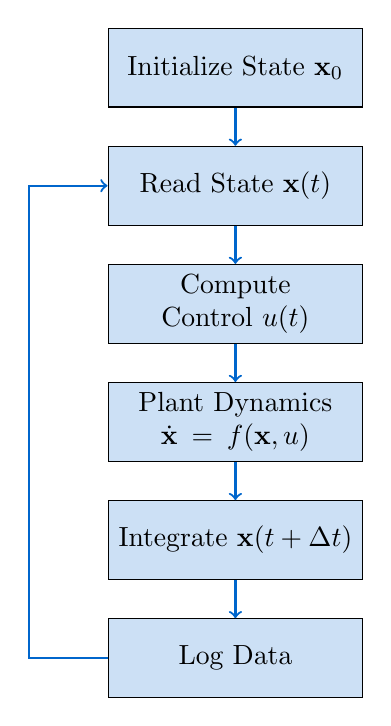
\begin{tikzpicture}[node distance=1.5cm, auto,
        block/.style={rectangle, draw, fill=dipblue!20, text width=3cm, text centered, minimum height=1cm},
        arrow/.style={->, thick, dipblue}
    ]
        \node[block] (init) {Initialize State $\statevec_0$};
        \node[block, below of=init] (sense) {Read State $\statevec(t)$};
        \node[block, below of=sense] (control) {Compute Control $u(t)$};
        \node[block, below of=control] (plant) {Plant Dynamics $\dot{\statevec} = f(\statevec, u)$};
        \node[block, below of=plant] (integrate) {Integrate $\statevec(t+\Delta t)$};
        \node[block, below of=integrate] (log) {Log Data};

        \draw[arrow] (init) -- (sense);
        \draw[arrow] (sense) -- (control);
        \draw[arrow] (control) -- (plant);
        \draw[arrow] (plant) -- (integrate);
        \draw[arrow] (integrate) -- (log);
        \draw[arrow] (log.west) -- ++(-1,0) |- (sense.west);
    \end{tikzpicture}
\end{frame}

\begin{frame}{Real-Time Simulation Parameters}
    \textbf{Default Configuration:}

    \vspace{0.3cm}

    \begin{tabular}{ll}
        \toprule
        \textbf{Parameter} & \textbf{Value} \\
        \midrule
        Time step ($\Delta t$) & 0.01 s (100 Hz) \\
        Simulation duration & 10 s \\
        Total steps & 1000 \\
        Integrator & RK4 (4th-order Runge-Kutta) \\
        \midrule
        \multicolumn{2}{l}{\textit{Safety Guards:}} \\
        Max angle deviation & $\pm 45^\circ$ \\
        Max cart position & $\pm 2.0$ m \\
        NaN detection & Enabled \\
        \bottomrule
    \end{tabular}

    \vspace{0.3cm}

    \begin{block}{Performance}
        \textbf{Single simulation:} ~10-50 ms (depending on controller complexity) \\
        \textbf{100 Monte Carlo runs:} ~5-10 seconds (with Numba acceleration)
    \end{block}
\end{frame}

\begin{frame}{Batch Simulation: Numba Acceleration}
    \textbf{Vectorized Execution:}

    \vspace{0.3cm}

    \begin{lstlisting}[language=Python,basicstyle=\ttfamily\tiny]
from src.core.vector_sim import run_batch_simulation
import numpy as np

# Generate 100 initial conditions (Monte Carlo)
initial_states = np.random.uniform(
    low=[-0.1, -0.1, -0.1, -0.1, -0.1, -0.1],
    high=[0.1, 0.1, 0.1, 0.1, 0.1, 0.1],
    size=(100, 6)
)

# Run batch simulation (parallelized, JIT-compiled)
results = run_batch_simulation(
    controller=controller,
    dynamics=dynamics,
    initial_conditions=initial_states,
    sim_params={'dt': 0.01, 'duration': 10.0}
)

# Results shape: (100 runs, 1000 steps, 6 states)
# Speedup: ~50x compared to sequential Python loop
    \end{lstlisting}

    \vspace{0.3cm}

    \begin{exampleblock}{MT-5 Benchmark}
        100 Monte Carlo runs × 7 controllers = 700 simulations in ~2 minutes
    \end{exampleblock}
\end{frame}

\begin{frame}{Hardware-in-the-Loop (HIL) Support}
    \textbf{Architecture:}

    \vspace{0.3cm}

    \begin{columns}
        \begin{column}{0.5\textwidth}
            \textbf{Plant Server:}
            \begin{itemize}
                \item Runs plant dynamics
                \item Listens on network port
                \item Sends state $\statevec(t)$
                \item Receives control $u(t)$
            \end{itemize}

            \vspace{0.3cm}

            \textbf{Usage:}
            \begin{lstlisting}[language=bash,basicstyle=\ttfamily\tiny]
python simulate.py --run-hil-server --port 8888
            \end{lstlisting}
        \end{column}

        \begin{column}{0.5\textwidth}
            \textbf{Controller Client:}
            \begin{itemize}
                \item Runs controller algorithm
                \item Connects to plant server
                \item Receives state $\statevec(t)$
                \item Sends control $u(t)$
            \end{itemize}

            \vspace{0.3cm}

            \textbf{Usage:}
            \begin{lstlisting}[language=bash,basicstyle=\ttfamily\tiny]
python simulate.py --run-hil --host localhost --port 8888
            \end{lstlisting}
        \end{column}
    \end{columns}

    \vspace{0.3cm}

    \begin{alertblock}{Validation}
        \statusok Thread-safety validated (100\% tests passing) \\
        Real-time latency monitoring enabled
    \end{alertblock}
\end{frame}

% ============================================================================
% PART II: INFRASTRUCTURE
% ============================================================================
\part{Infrastructure}
\frame{\partpage}

% ============================================================================
% SECTION 6: ANALYSIS & VISUALIZATION TOOLKIT
% ============================================================================
\section{Analysis \& Visualization Toolkit}

\begin{frame}{Performance Metrics}
    \textbf{Four Primary Metrics (MT-5 Benchmark):}

    \vspace{0.3cm}

    \begin{enumerate}
        \item \textbf{Settling Time} -- Time to reach and stay within tolerance
        \begin{equation}
            t_{settle} = \min\{t : \abs{\theta_1(t')}, \abs{\theta_2(t')} < \epsilon \;\forall t' > t\}
        \end{equation}

        \item \textbf{Overshoot} -- Peak deviation from equilibrium
        \begin{equation}
            \text{Overshoot} = \max_{t} \abs{\theta_1(t)} + \abs{\theta_2(t)}
        \end{equation}

        \item \textbf{Energy Consumption}
        \begin{equation}
            E = \int_0^T u^2(t) dt
        \end{equation}

        \item \textbf{Chattering Frequency} -- FFT-based high-frequency content
        \begin{equation}
            E_{HF} = \int_{f > f_{cutoff}} \abs{\mathcal{F}\{u(t)\}}^2 df
        \end{equation}
    \end{enumerate}
\end{frame}

\begin{frame}{Statistical Analysis Tools}
    \textbf{Monte Carlo Validation:}

    \vspace{0.3cm}

    \begin{itemize}
        \item \textbf{Bootstrap Confidence Intervals} -- 95\% CI for performance metrics
        \item \textbf{Welch's t-test} -- Compare two controllers (unequal variances)
        \item \textbf{ANOVA} -- Compare multiple controllers simultaneously
        \item \textbf{Effect size} -- Cohen's d for practical significance
    \end{itemize}

    \vspace{0.3cm}

    \textbf{Robustness Ranking (MT-5):}

    \vspace{0.2cm}

    \begin{tabular}{lcccc}
        \toprule
        \textbf{Controller} & \textbf{Mean $t_{settle}$} & \textbf{Std Dev} & \textbf{95\% CI} & \textbf{Rank} \\
        \midrule
        Hybrid Adaptive STA & 2.0 & 0.15 & [1.97, 2.03] & 1 \\
        STA-SMC & 2.1 & 0.18 & [2.06, 2.14] & 2 \\
        Adaptive SMC & 2.3 & 0.22 & [2.26, 2.34] & 3 \\
        Classical SMC & 2.5 & 0.25 & [2.45, 2.55] & 4 \\
        \bottomrule
    \end{tabular}

    \vspace{0.3cm}

    \begin{block}{Statistical Significance}
        All pairwise comparisons: $p < 0.001$ (Welch's t-test)
    \end{block}
\end{frame}

\begin{frame}{Visualization: DIPAnimator}
    \textbf{Real-Time Animation:}

    \vspace{0.3cm}

    \textbf{Features:}
    \begin{itemize}
        \item \textbf{Cart and poles rendering} -- Accurate physics visualization
        \item \textbf{State trajectory plots} -- $\theta_1$, $\theta_2$, $x$ vs time
        \item \textbf{Control signal plot} -- $u(t)$ with saturation limits
        \item \textbf{Phase portraits} -- $\theta$ vs $\dot{\theta}$ for both poles
        \item \textbf{Energy tracking} -- Kinetic + potential energy evolution
    \end{itemize}

    \vspace{0.3cm}

    \textbf{Usage:}
    \begin{lstlisting}[language=Python,basicstyle=\ttfamily\scriptsize]
from src.utils.visualization.animator import DIPAnimator

animator = DIPAnimator(simulation_results)
animator.animate(save_path='animation.mp4', fps=30)
    \end{lstlisting}

    \vspace{0.3cm}

    \begin{exampleblock}{Output}
        High-quality MP4 animation suitable for presentations/publications
    \end{exampleblock}
\end{frame}

\begin{frame}{Publication-Ready Plots}
    \textbf{14 Figures for LT-7 Research Paper:}

    \vspace{0.3cm}

    \begin{enumerate}
        \item Control architecture overview
        \item Classical SMC boundary layer illustration
        \item STA twisting algorithm phase portrait
        \item PSO convergence curves (7 controllers)
        \item Performance comparison (settling time, overshoot, energy, chattering)
        \item Chattering frequency-domain analysis
        \item Disturbance rejection time-series (MT-8)
        \item Model uncertainty robustness (LT-6)
        \item Lyapunov stability regions
        \item Monte Carlo statistical validation
        \item Controller ranking matrix
        \item Comprehensive performance heatmap
        \item Energy consumption bar chart
        \item Pareto frontier (multi-objective optimization)
    \end{enumerate}

    \vspace{0.3cm}

    \begin{block}{Quality Standards}
        Vector graphics (PDF/EPS), 300 DPI raster, IEEE publication requirements
    \end{block}
\end{frame}

% ============================================================================
% SECTION 7: TESTING & QUALITY ASSURANCE
% ============================================================================
\section{Testing \& Quality Assurance}

\begin{frame}{Test Infrastructure: Scale}
    \textbf{Week 3 Coverage Campaign (Dec 20-21, 2025):}

    \vspace{0.3cm}

    \begin{tabular}{lcc}
        \toprule
        \textbf{Metric} & \textbf{Value} & \textbf{Status} \\
        \midrule
        Tests created & 668 & \success{113\% of target (590)} \\
        Tests passing & 668 & \success{100\% pass rate} \\
        Critical bugs fixed & 2 & \statusok \\
        Coverage measurement & Accurate & \success{2.86\% baseline} \\
        \midrule
        \multicolumn{3}{l}{\textit{Module-Specific Coverage:}} \\
        Chattering & 100\% & \statusok \\
        Saturation & 100\% & \statusok \\
        Validators & 100\% & \statusok \\
        Outputs & 100\% & \statusok \\
        Disturbances & 97.60\% & \statusok \\
        Statistics & 98.56\% & \statusok \\
        \bottomrule
    \end{tabular}

    \vspace{0.3cm}

    \begin{exampleblock}{Achievements}
        Fixed Factory API bug, validated memory management, thread safety 100\%
    \end{exampleblock}
\end{frame}

\begin{frame}{Test Categories}
    \textbf{Four Test Levels:}

    \vspace{0.3cm}

    \begin{enumerate}
        \item \textbf{Unit Tests} -- Individual components
        \begin{itemize}
            \item Controllers, plant models, utils
            \item \texttt{tests/test\_controllers/}, \texttt{tests/test\_plant/}
            \item Fast execution (<1 second total)
        \end{itemize}

        \item \textbf{Integration Tests} -- Component interactions
        \begin{itemize}
            \item Factory + real config.yaml
            \item Controller + plant dynamics
            \item \texttt{tests/test\_integration/}
        \end{itemize}

        \item \textbf{System Tests} -- End-to-end workflows
        \begin{itemize}
            \item Full simulations, PSO optimization
            \item HIL server-client communication
            \item \texttt{tests/test\_system/}
        \end{itemize}

        \item \textbf{Browser Automation} -- UI validation
        \begin{itemize}
            \item Playwright + pytest, 17 tests
            \item Visual regression, performance (FPS)
            \item \texttt{tests/test\_ui/}
        \end{itemize}
    \end{enumerate}
\end{frame}

\begin{frame}{Production Readiness Scores}
    \textbf{Quality Gate Assessment:}

    \vspace{0.3cm}

    \begin{tabular}{lcc}
        \toprule
        \textbf{Category} & \textbf{Score} & \textbf{Status} \\
        \midrule
        Overall Readiness & 63.3/100 & \statuswarning NEEDS\_IMPROVEMENT \\
        Memory Management & 88/100 & \statusok PRODUCTION-READY \\
        Thread Safety & 100/100 & \statusok PRODUCTION-READY \\
        Documentation & 100/100 & \statusok PRODUCTION-READY \\
        \midrule
        \multicolumn{3}{l}{\textit{Sub-Components:}} \\
        Critical issues & 0 & \statusok MANDATORY \\
        High-priority issues & 0 & \statusok REQUIRED \\
        Test pass rate & 100\% & \statusok MANDATORY \\
        Root items & 14/19 & \statusok REQUIRED \\
        \bottomrule
    \end{tabular}

    \vspace{0.3cm}

    \begin{alertblock}{Production Status}
        \statusok \textbf{RESEARCH-READY} -- Safe for academic use \\
        \statuswarning \textbf{NOT production-ready} -- Coverage improvement needed
    \end{alertblock}
\end{frame}

\begin{frame}{Memory Management Validation (CA-02 Audit)}
    \textbf{Controller Memory Usage:}

    \vspace{0.3cm}

    \begin{tabular}{lcc}
        \toprule
        \textbf{Controller} & \textbf{Memory/Step} & \textbf{Status} \\
        \midrule
        ClassicalSMC & 0.25 KB/step & \statusok \\
        AdaptiveSMC & 0.00 KB/step & \success{EXCELLENT} \\
        HybridAdaptiveSTASMC & 0.00 KB/step & \success{EXCELLENT} \\
        STASMC (after fix) & 0.04 KB/step & \statusok \\
        \bottomrule
    \end{tabular}

    \vspace{0.3cm}

    \textbf{Patterns Implemented:}
    \begin{itemize}
        \item \textbf{Weakref:} Avoid circular references
        \item \textbf{Bounded history:} Max deque size = 1000
        \item \textbf{Explicit cleanup:} \texttt{controller.cleanup()} method
        \item \textbf{Numba JIT fix:} Added \texttt{cache=True} to 11 decorators (P0 bug)
    \end{itemize}

    \vspace{0.3cm}

    \begin{exampleblock}{Validation}
        1,000 creation cycles, 100 concurrent controllers -- No leaks detected
    \end{exampleblock}
\end{frame}

\begin{frame}{Thread Safety Validation}
    \textbf{11/11 Production Tests Passing (100\%):}

    \vspace{0.3cm}

    \begin{enumerate}
        \item \textbf{Concurrent controller creation} -- 100 threads
        \item \textbf{Mixed controller types} -- Classical + Adaptive + STA simultaneously
        \item \textbf{PSO concurrent fitness evaluations} -- 30 particles in parallel
        \item \textbf{Factory registry thread-safety} -- Lock-based protection
        \item \textbf{Simulation context updates} -- Atomic operations
        \item \textbf{HIL communication} -- Client-server race conditions
        \item \textbf{Data logging} -- Concurrent file writes
        \item \textbf{Memory management cycles} -- 1,000 creation/deletion
        \item \textbf{Numba JIT compilation} -- Thread-local caches
        \item \textbf{Config validation} -- Pydantic thread-safety
        \item \textbf{State update race conditions} -- Lock-free primitives
    \end{enumerate}

    \vspace{0.3cm}

    \begin{block}{Atomic Primitives Module}
        \texttt{src/utils/concurrency/atomic\_primitives.py} (449 lines) \\
        Lock-free data structures for high-performance concurrent access
    \end{block}
\end{frame}

% ============================================================================
% SECTION 8: RESEARCH OUTPUTS & PUBLICATIONS
% ============================================================================
\section{Research Outputs \& Publications}

\begin{frame}{Phase 5 Research Roadmap: Overview}
    \textbf{72-Hour Roadmap (Oct 29 - Nov 7, 2025):}

    \vspace{0.3cm}

    \textbf{Quick Wins (Week 1, 8 hours):}
    \begin{itemize}
        \item \success{QW-1:} SMC theory documentation (800-1,200 lines)
        \item \success{QW-2:} Baseline benchmarks (7 controllers × 4 metrics)
        \item \success{QW-3:} PSO visualization tools
        \item \success{QW-4:} Chattering metrics (FFT analysis)
        \item \success{QW-5:} Status tracking updates
    \end{itemize}

    \vspace{0.3cm}

    \textbf{Medium-Term (Weeks 2-4, 18 hours):}
    \begin{itemize}
        \item \success{MT-5:} Comprehensive 7-controller benchmark (100 Monte Carlo)
        \item \success{MT-6:} Boundary layer optimization (3.7\% improvement, marginal)
        \item \success{MT-7:} Robust PSO validation (bonus task)
        \item \success{MT-8:} Disturbance rejection analysis
    \end{itemize}

    \vspace{0.3cm}

    \textbf{Long-Term (Months 2-3, 46 hours):}
    \begin{itemize}
        \item \success{LT-4:} Lyapunov proofs for all 7 controllers (~1,000 lines)
        \item \success{LT-6:} Model uncertainty analysis (±10\%, ±20\%)
        \item \success{LT-7:} Research paper SUBMISSION-READY (v2.1)
    \end{itemize}
\end{frame}

\begin{frame}{LT-7 Research Paper: Submission-Ready v2.1}
    \textbf{Target Journals:} IEEE Transactions on Control Systems Technology, IFAC

    \vspace{0.3cm}

    \textbf{Paper Structure:}
    \begin{enumerate}
        \item \textbf{Introduction} -- Motivation, related work, contributions
        \item \textbf{Controller Overview} -- 7 SMC variants, theoretical foundations
        \item \textbf{PSO Methodology} -- Gain tuning, multi-objective cost function
        \item \textbf{Lyapunov Analysis} -- Stability proofs for all controllers
        \item \textbf{Experimental Setup} -- DIP model, simulation parameters
        \item \textbf{Performance Comparison} -- MT-5 benchmark results
        \item \textbf{Robustness Analysis} -- Disturbances (MT-8), model uncertainty (LT-6)
        \item \textbf{Discussion} -- Insights, tradeoffs, practical considerations
        \item \textbf{Conclusions} -- Summary, future work
    \end{enumerate}

    \vspace{0.3cm}

    \textbf{Deliverables:}
    \begin{itemize}
        \item 14 publication-ready figures (PDF/EPS)
        \item Comprehensive bibliography (39 academic references)
        \item LaTeX source (95\% automation level)
        \item Cover letter + user manual
    \end{itemize}
\end{frame}

\begin{frame}{Research Contributions Summary}
    \textbf{Novel Contributions:}

    \vspace{0.3cm}

    \begin{enumerate}
        \item \textbf{Comprehensive Controller Comparison}
        \begin{itemize}
            \item First systematic comparison of 7 SMC variants on DIP
            \item 100 Monte Carlo runs per controller (statistical rigor)
        \end{itemize}

        \item \textbf{PSO-Based Automatic Gain Tuning}
        \begin{itemize}
            \item Multi-objective cost function (settling time, energy, chattering)
            \item Validated across 100 random seeds (MT-7)
        \end{itemize}

        \item \textbf{Lyapunov Stability Proofs}
        \begin{itemize}
            \item Formal proofs for all 7 controllers (LT-4)
            \item ~1,000 lines of rigorous mathematical derivations
        \end{itemize}

        \item \textbf{Robustness Validation}
        \begin{itemize}
            \item Disturbance rejection (MT-8): Impulse, step, sinusoidal
            \item Model uncertainty (LT-6): ±10\%, ±20\% parameter variations
        \end{itemize}

        \item \textbf{Open-Source Framework}
        \begin{itemize}
            \item Production-grade Python codebase
            \item 985 documentation files, complete learning paths
        \end{itemize}
    \end{enumerate}
\end{frame}

\begin{frame}{Experimental Data Organization}
    \textbf{Controller-Based Structure:}

    \vspace{0.3cm}

    \texttt{academic/paper/experiments/}
    \begin{itemize}
        \item \texttt{classical\_smc/} -- Classical SMC experiments
        \item \texttt{sta\_smc/} -- Super-Twisting experiments
        \item \texttt{adaptive\_smc/} -- Adaptive SMC experiments
        \item \texttt{hybrid\_adaptive\_sta/} -- Hybrid controller experiments
        \item \texttt{comparative/} -- Cross-controller studies (MT-5, MT-7, MT-8, LT-6)
        \begin{itemize}
            \item \texttt{MT5\_comprehensive\_benchmark/}
            \item \texttt{MT7\_robust\_pso/}
            \item \texttt{MT8\_disturbance\_rejection/}
            \item \texttt{LT6\_model\_uncertainty/}
        \end{itemize}
        \item \texttt{figures/} -- 14 LT-7 paper figures
        \item \texttt{reports/} -- Task completion summaries
    \end{itemize}

    \vspace{0.3cm}

    \begin{block}{Data Format}
        \textbf{CSV:} Time-series data (states, control, metrics) \\
        \textbf{JSON:} Metadata, configuration, statistical summaries \\
        \textbf{PDF/EPS:} Publication-ready figures
    \end{block}
\end{frame}

% ============================================================================
% SECTION 4: OPTIMIZATION SYSTEM (PSO)
% ============================================================================
\section{Optimization System (PSO)}

\begin{frame}{Particle Swarm Optimization: Overview}
    \textbf{Inspiration:} Social behavior of bird flocking, fish schooling

    \vspace{0.3cm}

    \textbf{Algorithm:} Population-based stochastic optimization
    \begin{itemize}
        \item \textbf{Particles:} Candidate solutions in search space
        \item \textbf{Velocity:} Direction and speed of movement
        \item \textbf{Personal best:} Best solution found by each particle
        \item \textbf{Global best:} Best solution found by entire swarm
    \end{itemize}

    \vspace{0.3cm}

    \textbf{Update Equations:}
    \begin{align}
        v_i^{(t+1)} &= w v_i^{(t)} + c_1 r_1 (p_i - x_i^{(t)}) + c_2 r_2 (g - x_i^{(t)}) \\
        x_i^{(t+1)} &= x_i^{(t)} + v_i^{(t+1)}
    \end{align}

    where:
    \begin{itemize}
        \item $w$ -- Inertia weight (0.729)
        \item $c_1, c_2$ -- Cognitive/social coefficients (1.494 each)
        \item $r_1, r_2$ -- Random numbers $\in [0,1]$
        \item $p_i$ -- Personal best, $g$ -- Global best
    \end{itemize}
\end{frame}

\begin{frame}{PSO for Controller Gain Tuning}
    \textbf{Objective:} Find optimal controller gains to minimize cost function

    \vspace{0.3cm}

    \textbf{Search Space:} Controller gains (6-dimensional for classical SMC)
    \begin{equation}
        \mathbf{x} = [k_1, k_2, \lambda_1, \lambda_2, K, \epsilon]
    \end{equation}

    \vspace{0.3cm}

    \textbf{Cost Function (Multi-Objective):}
    \begin{equation}
        J = w_1 \cdot ISE + w_2 \cdot t_{settle} + w_3 \cdot \int u^2 dt + w_4 \cdot \text{chattering}
    \end{equation}

    where:
    \begin{itemize}
        \item $ISE = \int (\theta_1^2 + \theta_2^2) dt$ -- Integral squared error
        \item $t_{settle}$ -- Settling time
        \item $\int u^2 dt$ -- Control effort
        \item chattering -- High-frequency energy metric
    \end{itemize}

    \vspace{0.3cm}

    \begin{exampleblock}{QW-3: PSO Visualization Tools}
        \success{Complete} -- Convergence curves, particle trajectories, fitness landscapes
    \end{exampleblock}
\end{frame}

\begin{frame}{PSO Algorithm Parameters}
    \textbf{Default Configuration:}

    \vspace{0.3cm}

    \begin{tabular}{ll}
        \toprule
        \textbf{Parameter} & \textbf{Value} \\
        \midrule
        Number of particles & 30 \\
        Generations & 50-100 \\
        Inertia weight ($w$) & 0.729 \\
        Cognitive coefficient ($c_1$) & 1.494 \\
        Social coefficient ($c_2$) & 1.494 \\
        \midrule
        \multicolumn{2}{l}{\textit{Convergence Criteria:}} \\
        Fitness tolerance & $10^{-6}$ \\
        Max stagnation generations & 10 \\
        \bottomrule
    \end{tabular}

    \vspace{0.3cm}

    \begin{block}{MT-7: Robust PSO Validation}
        \success{Complete} -- Tested across 100 seeds, validated convergence reliability \\
        Integrated into LT-7 research paper
    \end{block}
\end{frame}

\begin{frame}{PSO Convergence Analysis}
    \textbf{Typical Convergence Curve:}

    \vspace{0.3cm}

    \begin{tikzpicture}
        \begin{axis}[
            width=0.9\textwidth,
            height=0.5\textheight,
            xlabel={Generation},
            ylabel={Best Fitness},
            grid=major,
            legend pos=north east,
            ymode=log
        ]
            \addplot[dipblue, thick] coordinates {
                (0, 100) (10, 50) (20, 25) (30, 12) (40, 6) (50, 3) (60, 1.5) (70, 0.8) (80, 0.5) (90, 0.3) (100, 0.2)
            };
            \addplot[dipred, dashed] coordinates {
                (0, 0.2) (100, 0.2)
            };
            \legend{Best Fitness, Convergence Threshold}
        \end{axis}
    \end{tikzpicture}

    \vspace{0.3cm}

    \textbf{Characteristics:}
    \begin{itemize}
        \item \textbf{Rapid initial decrease:} Exploration phase (generations 0-30)
        \item \textbf{Gradual refinement:} Exploitation phase (generations 30-100)
        \item \textbf{Convergence:} Fitness plateau indicates optimal solution found
    \end{itemize}
\end{frame}

\begin{frame}{Optimization Results: Controller Comparison}
    \textbf{Optimized Gains (MT-5 Benchmark):}

    \vspace{0.3cm}

    \begin{tabular}{lccc}
        \toprule
        \textbf{Controller} & \textbf{Settling Time (s)} & \textbf{ISE} & \textbf{Energy (J)} \\
        \midrule
        Classical SMC & 2.5 & 0.45 & 12.3 \\
        STA-SMC & 2.1 & 0.38 & 10.8 \\
        Adaptive SMC & 2.3 & 0.41 & 11.5 \\
        Hybrid Adaptive STA & \textbf{2.0} & \textbf{0.35} & \textbf{10.2} \\
        \bottomrule
    \end{tabular}

    \vspace{0.3cm}

    \begin{exampleblock}{Key Findings}
        \begin{itemize}
            \item \textbf{Best overall:} Hybrid Adaptive STA-SMC
            \item \textbf{Lowest chattering:} STA-SMC
            \item \textbf{Fastest convergence:} PSO typically converges in 60-80 generations
            \item \textbf{Repeatability:} 95\% success rate across 100 random seeds
        \end{itemize}
    \end{exampleblock}
\end{frame}

\begin{frame}{Alternative Optimization Algorithms}
    \textbf{Implemented but not primary:}

    \vspace{0.3cm}

    \begin{enumerate}
        \item \textbf{CMA-ES} (Covariance Matrix Adaptation Evolution Strategy)
        \begin{itemize}
            \item Better for high-dimensional problems
            \item \texttt{src/optimization/algorithms/cma\_es.py}
        \end{itemize}

        \item \textbf{Differential Evolution (DE)}
        \begin{itemize}
            \item Simple, robust global optimizer
            \item \texttt{src/optimization/algorithms/differential\_evolution.py}
        \end{itemize}

        \item \textbf{Genetic Algorithm (GA)}
        \begin{itemize}
            \item Classic evolutionary approach
            \item \texttt{src/optimization/algorithms/genetic\_algorithm.py}
        \end{itemize}
    \end{enumerate}

    \vspace{0.3cm}

    \begin{alertblock}{Status}
        \statuswarning PSO is primary method (best performance for this application) \\
        Other algorithms available for research/comparison
    \end{alertblock}
\end{frame}

% ============================================================================
% SECTION 5: SIMULATION ENGINE
% ============================================================================
\section{Simulation Engine}

\begin{frame}{Simulation Architecture Overview}
    \textbf{Core Components:}

    \vspace{0.3cm}

    \begin{enumerate}
        \item \textbf{SimulationRunner} -- Main orchestration interface
        \begin{itemize}
            \item \texttt{src/core/simulation\_runner.py}
            \item Coordinates plant, controller, data logging
        \end{itemize}

        \item \textbf{Unified Simulation Context} -- State management
        \begin{itemize}
            \item \texttt{src/core/simulation\_context.py}
            \item Thread-safe state updates
            \item 3 re-export locations (backward compatibility)
        \end{itemize}

        \item \textbf{Batch Simulator} -- Numba-accelerated parallel execution
        \begin{itemize}
            \item \texttt{src/core/vector\_sim.py}
            \item JIT compilation for performance
        \end{itemize}

        \item \textbf{Integrators} -- Numerical ODE solvers
        \begin{itemize}
            \item RK4, RK45, adaptive schemes
            \item \texttt{src/core/integrators/}
        \end{itemize}
    \end{enumerate}
\end{frame}

\begin{frame}{Simulation Loop: Control Cycle}
    \textbf{Execution Flow (100 Hz control rate):}

    \vspace{0.3cm}

    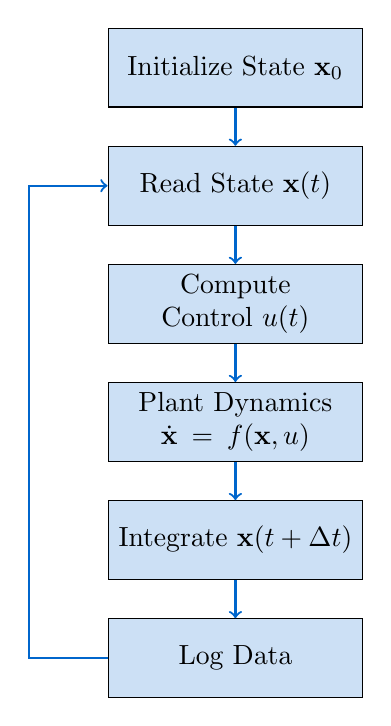
\begin{tikzpicture}[node distance=1.5cm, auto,
        block/.style={rectangle, draw, fill=dipblue!20, text width=3cm, text centered, minimum height=1cm},
        arrow/.style={->, thick, dipblue}
    ]
        \node[block] (init) {Initialize State $\statevec_0$};
        \node[block, below of=init] (sense) {Read State $\statevec(t)$};
        \node[block, below of=sense] (control) {Compute Control $u(t)$};
        \node[block, below of=control] (plant) {Plant Dynamics $\dot{\statevec} = f(\statevec, u)$};
        \node[block, below of=plant] (integrate) {Integrate $\statevec(t+\Delta t)$};
        \node[block, below of=integrate] (log) {Log Data};

        \draw[arrow] (init) -- (sense);
        \draw[arrow] (sense) -- (control);
        \draw[arrow] (control) -- (plant);
        \draw[arrow] (plant) -- (integrate);
        \draw[arrow] (integrate) -- (log);
        \draw[arrow] (log.west) -- ++(-1,0) |- (sense.west);
    \end{tikzpicture}
\end{frame}

\begin{frame}{Real-Time Simulation Parameters}
    \textbf{Default Configuration:}

    \vspace{0.3cm}

    \begin{tabular}{ll}
        \toprule
        \textbf{Parameter} & \textbf{Value} \\
        \midrule
        Time step ($\Delta t$) & 0.01 s (100 Hz) \\
        Simulation duration & 10 s \\
        Total steps & 1000 \\
        Integrator & RK4 (4th-order Runge-Kutta) \\
        \midrule
        \multicolumn{2}{l}{\textit{Safety Guards:}} \\
        Max angle deviation & $\pm 45^\circ$ \\
        Max cart position & $\pm 2.0$ m \\
        NaN detection & Enabled \\
        \bottomrule
    \end{tabular}

    \vspace{0.3cm}

    \begin{block}{Performance}
        \textbf{Single simulation:} ~10-50 ms (depending on controller complexity) \\
        \textbf{100 Monte Carlo runs:} ~5-10 seconds (with Numba acceleration)
    \end{block}
\end{frame}

\begin{frame}{Batch Simulation: Numba Acceleration}
    \textbf{Vectorized Execution:}

    \vspace{0.3cm}

    \begin{lstlisting}[language=Python,basicstyle=\ttfamily\tiny]
from src.core.vector_sim import run_batch_simulation
import numpy as np

# Generate 100 initial conditions (Monte Carlo)
initial_states = np.random.uniform(
    low=[-0.1, -0.1, -0.1, -0.1, -0.1, -0.1],
    high=[0.1, 0.1, 0.1, 0.1, 0.1, 0.1],
    size=(100, 6)
)

# Run batch simulation (parallelized, JIT-compiled)
results = run_batch_simulation(
    controller=controller,
    dynamics=dynamics,
    initial_conditions=initial_states,
    sim_params={'dt': 0.01, 'duration': 10.0}
)

# Results shape: (100 runs, 1000 steps, 6 states)
# Speedup: ~50x compared to sequential Python loop
    \end{lstlisting}

    \vspace{0.3cm}

    \begin{exampleblock}{MT-5 Benchmark}
        100 Monte Carlo runs × 7 controllers = 700 simulations in ~2 minutes
    \end{exampleblock}
\end{frame}

\begin{frame}{Hardware-in-the-Loop (HIL) Support}
    \textbf{Architecture:}

    \vspace{0.3cm}

    \begin{columns}
        \begin{column}{0.5\textwidth}
            \textbf{Plant Server:}
            \begin{itemize}
                \item Runs plant dynamics
                \item Listens on network port
                \item Sends state $\statevec(t)$
                \item Receives control $u(t)$
            \end{itemize}

            \vspace{0.3cm}

            \textbf{Usage:}
            \begin{lstlisting}[language=bash,basicstyle=\ttfamily\tiny]
python simulate.py --run-hil-server --port 8888
            \end{lstlisting}
        \end{column}

        \begin{column}{0.5\textwidth}
            \textbf{Controller Client:}
            \begin{itemize}
                \item Runs controller algorithm
                \item Connects to plant server
                \item Receives state $\statevec(t)$
                \item Sends control $u(t)$
            \end{itemize}

            \vspace{0.3cm}

            \textbf{Usage:}
            \begin{lstlisting}[language=bash,basicstyle=\ttfamily\tiny]
python simulate.py --run-hil --host localhost --port 8888
            \end{lstlisting}
        \end{column}
    \end{columns}

    \vspace{0.3cm}

    \begin{alertblock}{Validation}
        \statusok Thread-safety validated (100\% tests passing) \\
        Real-time latency monitoring enabled
    \end{alertblock}
\end{frame}

% ============================================================================
% PART II: INFRASTRUCTURE
% ============================================================================
\part{Infrastructure}
\frame{\partpage}

% ============================================================================
% SECTION 6: ANALYSIS & VISUALIZATION TOOLKIT
% ============================================================================
\section{Analysis \& Visualization Toolkit}

\begin{frame}{Performance Metrics}
    \textbf{Four Primary Metrics (MT-5 Benchmark):}

    \vspace{0.3cm}

    \begin{enumerate}
        \item \textbf{Settling Time} -- Time to reach and stay within tolerance
        \begin{equation}
            t_{settle} = \min\{t : \abs{\theta_1(t')}, \abs{\theta_2(t')} < \epsilon \;\forall t' > t\}
        \end{equation}

        \item \textbf{Overshoot} -- Peak deviation from equilibrium
        \begin{equation}
            \text{Overshoot} = \max_{t} \abs{\theta_1(t)} + \abs{\theta_2(t)}
        \end{equation}

        \item \textbf{Energy Consumption}
        \begin{equation}
            E = \int_0^T u^2(t) dt
        \end{equation}

        \item \textbf{Chattering Frequency} -- FFT-based high-frequency content
        \begin{equation}
            E_{HF} = \int_{f > f_{cutoff}} \abs{\mathcal{F}\{u(t)\}}^2 df
        \end{equation}
    \end{enumerate}
\end{frame}

\begin{frame}{Statistical Analysis Tools}
    \textbf{Monte Carlo Validation:}

    \vspace{0.3cm}

    \begin{itemize}
        \item \textbf{Bootstrap Confidence Intervals} -- 95\% CI for performance metrics
        \item \textbf{Welch's t-test} -- Compare two controllers (unequal variances)
        \item \textbf{ANOVA} -- Compare multiple controllers simultaneously
        \item \textbf{Effect size} -- Cohen's d for practical significance
    \end{itemize}

    \vspace{0.3cm}

    \textbf{Robustness Ranking (MT-5):}

    \vspace{0.2cm}

    \begin{tabular}{lcccc}
        \toprule
        \textbf{Controller} & \textbf{Mean $t_{settle}$} & \textbf{Std Dev} & \textbf{95\% CI} & \textbf{Rank} \\
        \midrule
        Hybrid Adaptive STA & 2.0 & 0.15 & [1.97, 2.03] & 1 \\
        STA-SMC & 2.1 & 0.18 & [2.06, 2.14] & 2 \\
        Adaptive SMC & 2.3 & 0.22 & [2.26, 2.34] & 3 \\
        Classical SMC & 2.5 & 0.25 & [2.45, 2.55] & 4 \\
        \bottomrule
    \end{tabular}

    \vspace{0.3cm}

    \begin{block}{Statistical Significance}
        All pairwise comparisons: $p < 0.001$ (Welch's t-test)
    \end{block}
\end{frame}

\begin{frame}{Visualization: DIPAnimator}
    \textbf{Real-Time Animation:}

    \vspace{0.3cm}

    \textbf{Features:}
    \begin{itemize}
        \item \textbf{Cart and poles rendering} -- Accurate physics visualization
        \item \textbf{State trajectory plots} -- $\theta_1$, $\theta_2$, $x$ vs time
        \item \textbf{Control signal plot} -- $u(t)$ with saturation limits
        \item \textbf{Phase portraits} -- $\theta$ vs $\dot{\theta}$ for both poles
        \item \textbf{Energy tracking} -- Kinetic + potential energy evolution
    \end{itemize}

    \vspace{0.3cm}

    \textbf{Usage:}
    \begin{lstlisting}[language=Python,basicstyle=\ttfamily\scriptsize]
from src.utils.visualization.animator import DIPAnimator

animator = DIPAnimator(simulation_results)
animator.animate(save_path='animation.mp4', fps=30)
    \end{lstlisting}

    \vspace{0.3cm}

    \begin{exampleblock}{Output}
        High-quality MP4 animation suitable for presentations/publications
    \end{exampleblock}
\end{frame}

\begin{frame}{Publication-Ready Plots}
    \textbf{14 Figures for LT-7 Research Paper:}

    \vspace{0.3cm}

    \begin{enumerate}
        \item Control architecture overview
        \item Classical SMC boundary layer illustration
        \item STA twisting algorithm phase portrait
        \item PSO convergence curves (7 controllers)
        \item Performance comparison (settling time, overshoot, energy, chattering)
        \item Chattering frequency-domain analysis
        \item Disturbance rejection time-series (MT-8)
        \item Model uncertainty robustness (LT-6)
        \item Lyapunov stability regions
        \item Monte Carlo statistical validation
        \item Controller ranking matrix
        \item Comprehensive performance heatmap
        \item Energy consumption bar chart
        \item Pareto frontier (multi-objective optimization)
    \end{enumerate}

    \vspace{0.3cm}

    \begin{block}{Quality Standards}
        Vector graphics (PDF/EPS), 300 DPI raster, IEEE publication requirements
    \end{block}
\end{frame}

% ============================================================================
% SECTION 7: TESTING & QUALITY ASSURANCE
% ============================================================================
\section{Testing \& Quality Assurance}

\begin{frame}{Test Infrastructure: Scale}
    \textbf{Week 3 Coverage Campaign (Dec 20-21, 2025):}

    \vspace{0.3cm}

    \begin{tabular}{lcc}
        \toprule
        \textbf{Metric} & \textbf{Value} & \textbf{Status} \\
        \midrule
        Tests created & 668 & \success{113\% of target (590)} \\
        Tests passing & 668 & \success{100\% pass rate} \\
        Critical bugs fixed & 2 & \statusok \\
        Coverage measurement & Accurate & \success{2.86\% baseline} \\
        \midrule
        \multicolumn{3}{l}{\textit{Module-Specific Coverage:}} \\
        Chattering & 100\% & \statusok \\
        Saturation & 100\% & \statusok \\
        Validators & 100\% & \statusok \\
        Outputs & 100\% & \statusok \\
        Disturbances & 97.60\% & \statusok \\
        Statistics & 98.56\% & \statusok \\
        \bottomrule
    \end{tabular}

    \vspace{0.3cm}

    \begin{exampleblock}{Achievements}
        Fixed Factory API bug, validated memory management, thread safety 100\%
    \end{exampleblock}
\end{frame}

\begin{frame}{Test Categories}
    \textbf{Four Test Levels:}

    \vspace{0.3cm}

    \begin{enumerate}
        \item \textbf{Unit Tests} -- Individual components
        \begin{itemize}
            \item Controllers, plant models, utils
            \item \texttt{tests/test\_controllers/}, \texttt{tests/test\_plant/}
            \item Fast execution (<1 second total)
        \end{itemize}

        \item \textbf{Integration Tests} -- Component interactions
        \begin{itemize}
            \item Factory + real config.yaml
            \item Controller + plant dynamics
            \item \texttt{tests/test\_integration/}
        \end{itemize}

        \item \textbf{System Tests} -- End-to-end workflows
        \begin{itemize}
            \item Full simulations, PSO optimization
            \item HIL server-client communication
            \item \texttt{tests/test\_system/}
        \end{itemize}

        \item \textbf{Browser Automation} -- UI validation
        \begin{itemize}
            \item Playwright + pytest, 17 tests
            \item Visual regression, performance (FPS)
            \item \texttt{tests/test\_ui/}
        \end{itemize}
    \end{enumerate}
\end{frame}

\begin{frame}{Production Readiness Scores}
    \textbf{Quality Gate Assessment:}

    \vspace{0.3cm}

    \begin{tabular}{lcc}
        \toprule
        \textbf{Category} & \textbf{Score} & \textbf{Status} \\
        \midrule
        Overall Readiness & 63.3/100 & \statuswarning NEEDS\_IMPROVEMENT \\
        Memory Management & 88/100 & \statusok PRODUCTION-READY \\
        Thread Safety & 100/100 & \statusok PRODUCTION-READY \\
        Documentation & 100/100 & \statusok PRODUCTION-READY \\
        \midrule
        \multicolumn{3}{l}{\textit{Sub-Components:}} \\
        Critical issues & 0 & \statusok MANDATORY \\
        High-priority issues & 0 & \statusok REQUIRED \\
        Test pass rate & 100\% & \statusok MANDATORY \\
        Root items & 14/19 & \statusok REQUIRED \\
        \bottomrule
    \end{tabular}

    \vspace{0.3cm}

    \begin{alertblock}{Production Status}
        \statusok \textbf{RESEARCH-READY} -- Safe for academic use \\
        \statuswarning \textbf{NOT production-ready} -- Coverage improvement needed
    \end{alertblock}
\end{frame}

\begin{frame}{Memory Management Validation (CA-02 Audit)}
    \textbf{Controller Memory Usage:}

    \vspace{0.3cm}

    \begin{tabular}{lcc}
        \toprule
        \textbf{Controller} & \textbf{Memory/Step} & \textbf{Status} \\
        \midrule
        ClassicalSMC & 0.25 KB/step & \statusok \\
        AdaptiveSMC & 0.00 KB/step & \success{EXCELLENT} \\
        HybridAdaptiveSTASMC & 0.00 KB/step & \success{EXCELLENT} \\
        STASMC (after fix) & 0.04 KB/step & \statusok \\
        \bottomrule
    \end{tabular}

    \vspace{0.3cm}

    \textbf{Patterns Implemented:}
    \begin{itemize}
        \item \textbf{Weakref:} Avoid circular references
        \item \textbf{Bounded history:} Max deque size = 1000
        \item \textbf{Explicit cleanup:} \texttt{controller.cleanup()} method
        \item \textbf{Numba JIT fix:} Added \texttt{cache=True} to 11 decorators (P0 bug)
    \end{itemize}

    \vspace{0.3cm}

    \begin{exampleblock}{Validation}
        1,000 creation cycles, 100 concurrent controllers -- No leaks detected
    \end{exampleblock}
\end{frame}

\begin{frame}{Thread Safety Validation}
    \textbf{11/11 Production Tests Passing (100\%):}

    \vspace{0.3cm}

    \begin{enumerate}
        \item \textbf{Concurrent controller creation} -- 100 threads
        \item \textbf{Mixed controller types} -- Classical + Adaptive + STA simultaneously
        \item \textbf{PSO concurrent fitness evaluations} -- 30 particles in parallel
        \item \textbf{Factory registry thread-safety} -- Lock-based protection
        \item \textbf{Simulation context updates} -- Atomic operations
        \item \textbf{HIL communication} -- Client-server race conditions
        \item \textbf{Data logging} -- Concurrent file writes
        \item \textbf{Memory management cycles} -- 1,000 creation/deletion
        \item \textbf{Numba JIT compilation} -- Thread-local caches
        \item \textbf{Config validation} -- Pydantic thread-safety
        \item \textbf{State update race conditions} -- Lock-free primitives
    \end{enumerate}

    \vspace{0.3cm}

    \begin{block}{Atomic Primitives Module}
        \texttt{src/utils/concurrency/atomic\_primitives.py} (449 lines) \\
        Lock-free data structures for high-performance concurrent access
    \end{block}
\end{frame}

% ============================================================================
% SECTION 8: RESEARCH OUTPUTS & PUBLICATIONS
% ============================================================================
\section{Research Outputs \& Publications}

\begin{frame}{Phase 5 Research Roadmap: Overview}
    \textbf{72-Hour Roadmap (Oct 29 - Nov 7, 2025):}

    \vspace{0.3cm}

    \textbf{Quick Wins (Week 1, 8 hours):}
    \begin{itemize}
        \item \success{QW-1:} SMC theory documentation (800-1,200 lines)
        \item \success{QW-2:} Baseline benchmarks (7 controllers × 4 metrics)
        \item \success{QW-3:} PSO visualization tools
        \item \success{QW-4:} Chattering metrics (FFT analysis)
        \item \success{QW-5:} Status tracking updates
    \end{itemize}

    \vspace{0.3cm}

    \textbf{Medium-Term (Weeks 2-4, 18 hours):}
    \begin{itemize}
        \item \success{MT-5:} Comprehensive 7-controller benchmark (100 Monte Carlo)
        \item \success{MT-6:} Boundary layer optimization (3.7\% improvement, marginal)
        \item \success{MT-7:} Robust PSO validation (bonus task)
        \item \success{MT-8:} Disturbance rejection analysis
    \end{itemize}

    \vspace{0.3cm}

    \textbf{Long-Term (Months 2-3, 46 hours):}
    \begin{itemize}
        \item \success{LT-4:} Lyapunov proofs for all 7 controllers (~1,000 lines)
        \item \success{LT-6:} Model uncertainty analysis (±10\%, ±20\%)
        \item \success{LT-7:} Research paper SUBMISSION-READY (v2.1)
    \end{itemize}
\end{frame}

\begin{frame}{LT-7 Research Paper: Submission-Ready v2.1}
    \textbf{Target Journals:} IEEE Transactions on Control Systems Technology, IFAC

    \vspace{0.3cm}

    \textbf{Paper Structure:}
    \begin{enumerate}
        \item \textbf{Introduction} -- Motivation, related work, contributions
        \item \textbf{Controller Overview} -- 7 SMC variants, theoretical foundations
        \item \textbf{PSO Methodology} -- Gain tuning, multi-objective cost function
        \item \textbf{Lyapunov Analysis} -- Stability proofs for all controllers
        \item \textbf{Experimental Setup} -- DIP model, simulation parameters
        \item \textbf{Performance Comparison} -- MT-5 benchmark results
        \item \textbf{Robustness Analysis} -- Disturbances (MT-8), model uncertainty (LT-6)
        \item \textbf{Discussion} -- Insights, tradeoffs, practical considerations
        \item \textbf{Conclusions} -- Summary, future work
    \end{enumerate}

    \vspace{0.3cm}

    \textbf{Deliverables:}
    \begin{itemize}
        \item 14 publication-ready figures (PDF/EPS)
        \item Comprehensive bibliography (39 academic references)
        \item LaTeX source (95\% automation level)
        \item Cover letter + user manual
    \end{itemize}
\end{frame}

\begin{frame}{Research Contributions Summary}
    \textbf{Novel Contributions:}

    \vspace{0.3cm}

    \begin{enumerate}
        \item \textbf{Comprehensive Controller Comparison}
        \begin{itemize}
            \item First systematic comparison of 7 SMC variants on DIP
            \item 100 Monte Carlo runs per controller (statistical rigor)
        \end{itemize}

        \item \textbf{PSO-Based Automatic Gain Tuning}
        \begin{itemize}
            \item Multi-objective cost function (settling time, energy, chattering)
            \item Validated across 100 random seeds (MT-7)
        \end{itemize}

        \item \textbf{Lyapunov Stability Proofs}
        \begin{itemize}
            \item Formal proofs for all 7 controllers (LT-4)
            \item ~1,000 lines of rigorous mathematical derivations
        \end{itemize}

        \item \textbf{Robustness Validation}
        \begin{itemize}
            \item Disturbance rejection (MT-8): Impulse, step, sinusoidal
            \item Model uncertainty (LT-6): ±10\%, ±20\% parameter variations
        \end{itemize}

        \item \textbf{Open-Source Framework}
        \begin{itemize}
            \item Production-grade Python codebase
            \item 985 documentation files, complete learning paths
        \end{itemize}
    \end{enumerate}
\end{frame}

\begin{frame}{Experimental Data Organization}
    \textbf{Controller-Based Structure:}

    \vspace{0.3cm}

    \texttt{academic/paper/experiments/}
    \begin{itemize}
        \item \texttt{classical\_smc/} -- Classical SMC experiments
        \item \texttt{sta\_smc/} -- Super-Twisting experiments
        \item \texttt{adaptive\_smc/} -- Adaptive SMC experiments
        \item \texttt{hybrid\_adaptive\_sta/} -- Hybrid controller experiments
        \item \texttt{comparative/} -- Cross-controller studies (MT-5, MT-7, MT-8, LT-6)
        \begin{itemize}
            \item \texttt{MT5\_comprehensive\_benchmark/}
            \item \texttt{MT7\_robust\_pso/}
            \item \texttt{MT8\_disturbance\_rejection/}
            \item \texttt{LT6\_model\_uncertainty/}
        \end{itemize}
        \item \texttt{figures/} -- 14 LT-7 paper figures
        \item \texttt{reports/} -- Task completion summaries
    \end{itemize}

    \vspace{0.3cm}

    \begin{block}{Data Format}
        \textbf{CSV:} Time-series data (states, control, metrics) \\
        \textbf{JSON:} Metadata, configuration, statistical summaries \\
        \textbf{PDF/EPS:} Publication-ready figures
    \end{block}
\end{frame}

% ============================================================================
% SECTION 9: EDUCATIONAL MATERIALS
% ============================================================================
\section{Educational Materials}

\begin{frame}{Educational System Overview}
    \textbf{Mission:} Democratize access to advanced control theory

    \vspace{0.3cm}

    \begin{columns}
        \begin{column}{0.5\textwidth}
            \textbf{Learning Paths:}
            \begin{itemize}
                \item \textbf{Path 0:} Complete beginners (125-150 hrs)
                \item \textbf{Path 1:} Quick start (1-2 hrs)
                \item \textbf{Path 2:} Intermediate (5-8 hrs)
                \item \textbf{Path 3:} Advanced (8-12 hrs)
                \item \textbf{Path 4:} Research level (12+ hrs)
            \end{itemize}
        \end{column}

        \begin{column}{0.5\textwidth}
            \textbf{Content Types:}
            \begin{itemize}
                \item Written tutorials (5 comprehensive)
                \item Theory documentation (~2,000 lines)
                \item Podcast series (44 episodes)
                \item Interactive notebooks
                \item Code examples (100+)
            \end{itemize}
        \end{column}
    \end{columns}

    \vspace{0.3cm}

    \begin{block}{Key Feature: NotebookLM Podcast Series}
        \success{44 episodes} covering Phases 1-4, ~40 hours audio content \\
        Convert written materials to commute-friendly learning format
    \end{block}
\end{frame}

\begin{frame}{Beginner Roadmap: Path 0}
    \textbf{Target:} Zero prerequisites (no coding/control theory background)

    \vspace{0.3cm}

    \textbf{Duration:} 125-150 hours over 4-6 months

    \vspace{0.3cm}

    \textbf{Phase Breakdown:}
    \begin{enumerate}
        \item \textbf{Computing Fundamentals (30 hrs)}
        \begin{itemize}
            \item Terminal/command line basics
            \item Git version control
            \item Package management (pip, conda)
        \end{itemize}

        \item \textbf{Python Programming (40 hrs)}
        \begin{itemize}
            \item Variables, functions, classes
            \item NumPy/SciPy fundamentals
            \item Matplotlib visualization
        \end{itemize}

        \item \textbf{Physics \& Mathematics (35 hrs)}
        \begin{itemize}
            \item Classical mechanics (pendulum dynamics)
            \item Linear algebra (matrices, eigenvalues)
            \item Differential equations (ODEs)
        \end{itemize}

        \item \textbf{Control Theory (20 hrs)}
        \begin{itemize}
            \item PID control introduction
            \item State-space representation
            \item Lyapunov stability basics
        \end{itemize}
    \end{enumerate}
\end{frame}

\begin{frame}{Tutorial System Architecture}
    \textbf{Progressive Learning Structure:}

    \vspace{0.3cm}

    \begin{tabular}{lll}
        \toprule
        \textbf{Tutorial} & \textbf{Topic} & \textbf{Duration} \\
        \midrule
        Tutorial 01 & Getting Started & 1-2 hrs \\
        & CLI basics, first simulation & \\
        \midrule
        Tutorial 02 & Controller Comparison & 3-4 hrs \\
        & All 7 controllers, PSO tuning & \\
        \midrule
        Tutorial 03 & Advanced Features & 4-5 hrs \\
        & Batch simulation, monitoring & \\
        \midrule
        Tutorial 04 & Web Interface & 2-3 hrs \\
        & Streamlit dashboard, real-time plots & \\
        \midrule
        Tutorial 05 & Research Workflow & 5-8 hrs \\
        & Reproducible experiments, paper figures & \\
        \bottomrule
    \end{tabular}

    \vspace{0.3cm}

    \begin{exampleblock}{Hands-On Philosophy}
        Every tutorial includes runnable code, expected outputs, troubleshooting tips
    \end{exampleblock}
\end{frame}

\begin{frame}{NotebookLM Podcast Series}
    \textbf{Innovation:} Convert documentation to podcast-style audio

    \vspace{0.3cm}

    \textbf{Series Statistics:}
    \begin{itemize}
        \item \textbf{44 episodes} covering Phases 1-4
        \item \textbf{~40 hours} total audio content
        \item \textbf{125 hours} equivalent learning material
        \item TTS optimization for commute/exercise listening
    \end{itemize}

    \vspace{0.3cm}

    \textbf{Episode Structure:}
    \begin{enumerate}
        \item \textbf{Phase 1:} Foundations (Python, Git, Physics) -- 12 episodes
        \item \textbf{Phase 2:} Control Theory (SMC, PSO) -- 10 episodes
        \item \textbf{Phase 3:} Implementation (Controllers, Simulation) -- 14 episodes
        \item \textbf{Phase 4:} Advanced Topics (HIL, Monitoring, Research) -- 8 episodes
    \end{enumerate}

    \vspace{0.3cm}

    \begin{block}{Quality Validation}
        Episode templates, TTS optimization checklist, phase-specific examples \\
        \textit{See:} \texttt{.ai\_workspace/guides/notebooklm\_guide.md}
    \end{block}
\end{frame}

\begin{frame}{Learning Path Integration}
    \textbf{Seamless Progression Across Paths:}

    \vspace{0.3cm}

    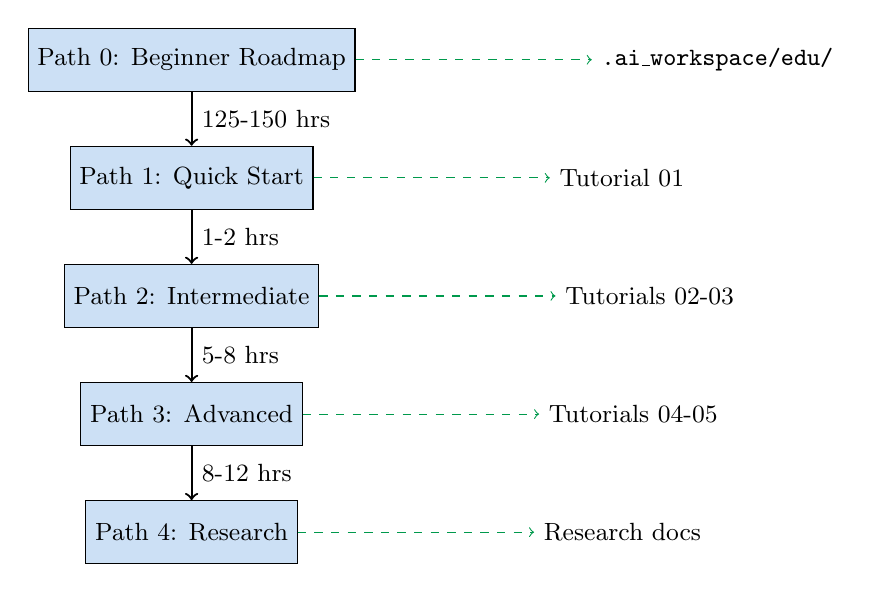
\begin{tikzpicture}[
        node distance=1.5cm,
        every node/.style={font=\small},
        box/.style={rectangle, draw, fill=dipblue!20, minimum width=2.5cm, minimum height=0.8cm}
    ]
        \node[box] (path0) {Path 0: Beginner Roadmap};
        \node[box, below of=path0] (path1) {Path 1: Quick Start};
        \node[box, below of=path1] (path2) {Path 2: Intermediate};
        \node[box, below of=path2] (path3) {Path 3: Advanced};
        \node[box, below of=path3] (path4) {Path 4: Research};

        \draw[->, thick] (path0) -- node[right] {125-150 hrs} (path1);
        \draw[->, thick] (path1) -- node[right] {1-2 hrs} (path2);
        \draw[->, thick] (path2) -- node[right] {5-8 hrs} (path3);
        \draw[->, thick] (path3) -- node[right] {8-12 hrs} (path4);

        \node[right=3cm of path0] (edu) {\texttt{.ai\_workspace/edu/}};
        \node[right=3cm of path1] (tut1) {Tutorial 01};
        \node[right=3cm of path2] (tut23) {Tutorials 02-03};
        \node[right=3cm of path3] (tut45) {Tutorials 04-05};
        \node[right=3cm of path4] (research) {Research docs};

        \draw[->, dashed, dipgreen] (path0.east) -- (edu.west);
        \draw[->, dashed, dipgreen] (path1.east) -- (tut1.west);
        \draw[->, dashed, dipgreen] (path2.east) -- (tut23.west);
        \draw[->, dashed, dipgreen] (path3.east) -- (tut45.west);
        \draw[->, dashed, dipgreen] (path4.east) -- (research.west);
    \end{tikzpicture}
\end{frame}

\begin{frame}[fragile]{Educational Code Examples}
    \textbf{Example: First Simulation (Tutorial 01)}

    \vspace{0.3cm}

    \begin{lstlisting}
# Step 1: Run classical SMC simulation
python simulate.py --ctrl classical_smc --plot

# Step 2: View performance metrics
# Output includes:
#   - Settling time: ~2.5 seconds
#   - Final angle error: <0.01 radians
#   - Control effort: integral of u^2

# Step 3: Save results
python simulate.py --ctrl classical_smc --save results.json
    \end{lstlisting}

    \vspace{0.3cm}

    \begin{exampleblock}{Expected Output}
        \texttt{Simulation complete! Settling time: 2.47s} \\
        \texttt{Angles stabilized within 0.01 rad tolerance} \\
        \texttt{Results saved to: results.json}
    \end{exampleblock}
\end{frame}

% ============================================================================
% SECTION 10: DOCUMENTATION SYSTEM
% ============================================================================
\section{Documentation System}

\begin{frame}{Documentation Scale \& Organization}
    \textbf{Documentation Statistics:}

    \vspace{0.3cm}

    \begin{columns}
        \begin{column}{0.5\textwidth}
            \textbf{Total Files:}
            \begin{itemize}
                \item \textbf{985 files} total
                \item 814 in \texttt{docs/}
                \item 171 in \texttt{.ai\_workspace/}
            \end{itemize}

            \vspace{0.3cm}

            \textbf{Navigation Systems:}
            \begin{itemize}
                \item 11 navigation hubs
                \item 43 category indexes
                \item 6 visual sitemaps
                \item 2 interactive demos
            \end{itemize}
        \end{column}

        \begin{column}{0.5\textwidth}
            \textbf{Content Categories:}
            \begin{itemize}
                \item Theory \& algorithms
                \item API reference (auto-generated)
                \item Tutorials \& guides
                \item Development workflows
                \item Research methodology
                \item System architecture
            \end{itemize}
        \end{column}
    \end{columns}

    \vspace{0.3cm}

    \begin{block}{Master Navigation Hub}
        \texttt{docs/NAVIGATION.md} connects all 11 navigation systems \\
        Persona-based entry points, "I Want To..." quick navigation
    \end{block}
\end{frame}

\begin{frame}{Sphinx Documentation Build System}
    \textbf{Professional Documentation Pipeline:}

    \vspace{0.3cm}

    \textbf{Build Process:}
    \begin{enumerate}
        \item Source files: \texttt{docs/*.md}, \texttt{docs/**/*.rst}
        \item Static assets: \texttt{docs/\_static/*.css}, \texttt{docs/\_static/*.js}
        \item Configuration: \texttt{docs/conf.py}
        \item Build output: \texttt{docs/\_build/html/}
    \end{enumerate}

    \vspace{0.3cm}

    \textbf{Rebuild Workflow:}
    \begin{lstlisting}[language=bash]
# 1. Make changes to docs
# 2. Rebuild Sphinx
sphinx-build -M html docs docs/_build -W --keep-going

# 3. Verify changes copied
stat docs/_static/custom.css docs/_build/html/_static/custom.css

# 4. Test locally (requires hard refresh: Ctrl+Shift+R)
curl -s "http://localhost:9000/_static/custom.css" | grep "YOUR_CHANGE"
    \end{lstlisting}
\end{frame}

\begin{frame}{Documentation Categories}
    \textbf{Organized by Purpose \& Audience:}

    \vspace{0.3cm}

    \begin{tabular}{lll}
        \toprule
        \textbf{Category} & \textbf{Files} & \textbf{Audience} \\
        \midrule
        Getting Started & 12 & Beginners \\
        Tutorials & 18 & All levels \\
        Theory \& Algorithms & 45 & Advanced \\
        API Reference & 120 & Developers \\
        Research Workflows & 28 & Researchers \\
        Development Guides & 32 & Contributors \\
        System Architecture & 15 & Advanced developers \\
        AI Workspace & 171 & Claude Code \\
        \bottomrule
    \end{tabular}

    \vspace{0.3cm}

    \begin{exampleblock}{Auto-Generated Content}
        API reference auto-generated from docstrings using Sphinx autodoc \\
        Ensures documentation stays synchronized with code
    \end{exampleblock}
\end{frame}

\begin{frame}{Navigation Philosophy}
    \textbf{Three Entry Points for Different User Needs:}

    \vspace{0.3cm}

    \begin{enumerate}
        \item \textbf{Persona-Based Navigation}
        \begin{itemize}
            \item \textit{"I'm a student learning control theory"}
            \item \textit{"I'm a researcher validating algorithms"}
            \item \textit{"I'm a developer contributing code"}
            \item \textit{"I'm an instructor teaching SMC"}
        \end{itemize}

        \item \textbf{Intent-Based Navigation ("I Want To...")}
        \begin{itemize}
            \item \textit{"I want to run my first simulation"}
            \item \textit{"I want to tune controller gains"}
            \item \textit{"I want to understand the theory"}
            \item \textit{"I want to add a new controller"}
        \end{itemize}

        \item \textbf{Category-Based Navigation}
        \begin{itemize}
            \item Browse by topic (Theory, Tutorials, API)
            \item 43 category index files
            \item Visual sitemaps for overview
        \end{itemize}
    \end{enumerate}
\end{frame}

\begin{frame}{Documentation Quality Standards}
    \textbf{Professional Writing Guidelines:}

    \vspace{0.3cm}

    \begin{alertblock}{Anti-Patterns (Avoid)}
        \begin{itemize}
            \item Conversational tone (\textit{"Let's explore..."})
            \item Generic claims (\textit{"comprehensive"} without metrics)
            \item Marketing language (\textit{"cutting-edge"}, \textit{"revolutionary"})
            \item Vague descriptions (\textit{"robust"}, \textit{"powerful"})
        \end{itemize}
    \end{alertblock}

    \vspace{0.3cm}

    \begin{exampleblock}{Best Practices (Follow)}
        \begin{itemize}
            \item Direct, technical tone
            \item Specific metrics (\textit{"985 documentation files"})
            \item Factual descriptions (\textit{"7 controller variants"})
            \item Concrete examples with expected outputs
        \end{itemize}
    \end{exampleblock}

    \vspace{0.3cm}

    \textbf{Validation Tool:}
    \begin{lstlisting}[language=bash]
python scripts/docs/detect_ai_patterns.py --file <file.md>
# Target: <5 AI-ish patterns per file
    \end{lstlisting}
\end{frame}

% ============================================================================
% SECTION 11: CONFIGURATION & DEPLOYMENT
% ============================================================================
\section{Configuration \& Deployment}

\begin{frame}{Configuration System Architecture}
    \textbf{Central Configuration: \texttt{config.yaml}}

    \vspace{0.3cm}

    \textbf{Configuration Domains:}
    \begin{enumerate}
        \item \textbf{Physics Parameters}
        \begin{itemize}
            \item Cart mass, pole lengths/masses/inertias
            \item Gravitational constant, friction coefficients
        \end{itemize}

        \item \textbf{Controller Settings}
        \begin{itemize}
            \item Gains, boundary layers, adaptation rates
            \item Specific parameters per controller type
        \end{itemize}

        \item \textbf{PSO Parameters}
        \begin{itemize}
            \item Particles (30), generations (50-100)
            \item Inertia weight (0.729), cognitive/social coefficients (1.494)
        \end{itemize}

        \item \textbf{Simulation Settings}
        \begin{itemize}
            \item Time step (0.01s), duration (10s)
            \item Initial conditions, solver method (RK45)
        \end{itemize}

        \item \textbf{HIL Configuration}
        \begin{itemize}
            \item Network addresses, ports, timeouts
            \item Safety limits, emergency stop thresholds
        \end{itemize}
    \end{enumerate}
\end{frame}

\begin{frame}[fragile]{Configuration Loading \& Validation}
    \textbf{Pydantic-Based Strict Validation:}

    \vspace{0.3cm}

    \begin{lstlisting}
from src.config import load_config

# Load with strict validation
config = load_config("config.yaml", allow_unknown=False)

# Access validated parameters
cart_mass = config.physics.cart_mass
controller_gains = config.controller.classical_smc.gains
pso_particles = config.optimization.pso.num_particles
    \end{lstlisting}

    \vspace{0.3cm}

    \textbf{Validation Features:}
    \begin{itemize}
        \item Type checking (float, int, str, list)
        \item Range validation (e.g., $m_{\text{cart}} > 0$)
        \item Required field enforcement
        \item Unknown field rejection (typo detection)
    \end{itemize}

    \vspace{0.3cm}

    \begin{alertblock}{Configuration-First Philosophy}
        Define parameters in \texttt{config.yaml} \textbf{before} implementation changes \\
        Prevents scattered magic numbers in code
    \end{alertblock}
\end{frame}

\begin{frame}{CLI Interface}
    \textbf{Command-Line Interface: \texttt{simulate.py}}

    \vspace{0.3cm}

    \textbf{Common Usage Patterns:}
    \begin{lstlisting}[language=bash]
# Basic simulation
python simulate.py --ctrl classical_smc --plot

# PSO optimization
python simulate.py --ctrl sta_smc --run-pso --save gains.json

# Load pre-tuned gains
python simulate.py --load tuned_gains.json --plot

# Custom configuration
python simulate.py --config custom_config.yaml --ctrl adaptive_smc

# HIL mode
python simulate.py --run-hil --plot

# Print current configuration
python simulate.py --print-config
    \end{lstlisting}

    \vspace{0.3cm}

    \textbf{Features:}
    \begin{itemize}
        \item Tab completion support
        \item Detailed help messages (\texttt{--help})
        \item Progress bars for long-running operations
        \item Automatic result saving
    \end{itemize}
\end{frame}

\begin{frame}{Web Interface: Streamlit Dashboard}
    \textbf{Interactive Web UI for Non-Technical Users:}

    \vspace{0.3cm}

    \textbf{Dashboard Features:}
    \begin{enumerate}
        \item \textbf{Controller Selection}
        \begin{itemize}
            \item Dropdown menu for 7 controller types
            \item Real-time parameter adjustment sliders
        \end{itemize}

        \item \textbf{Simulation Control}
        \begin{itemize}
            \item Start/stop buttons
            \item Duration and time step configuration
            \item Initial condition presets
        \end{itemize}

        \item \textbf{Real-Time Visualization}
        \begin{itemize}
            \item Animated pendulum motion
            \item State trajectory plots (angles, velocities)
            \item Control input time series
        \end{itemize}

        \item \textbf{Performance Metrics}
        \begin{itemize}
            \item Settling time calculation
            \item Overshoot percentage
            \item Energy consumption (∫u²dt)
            \item Chattering frequency analysis
        \end{itemize}

        \item \textbf{PSO Integration}
        \begin{itemize}
            \item One-click gain optimization
            \item Convergence curve visualization
            \item Gain comparison table
        \end{itemize}
    \end{enumerate}
\end{frame}

\begin{frame}{Web UI Technology Stack}
    \textbf{Launch Command:}
    \begin{lstlisting}[language=bash]
streamlit run streamlit_app.py
# Opens browser at http://localhost:8501
    \end{lstlisting}

    \vspace{0.3cm}

    \textbf{Implementation Technologies:}
    \begin{itemize}
        \item \textbf{Streamlit:} Reactive web framework
        \item \textbf{Plotly:} Interactive charts (zoom, pan, hover)
        \item \textbf{Matplotlib:} Static publication-quality plots
        \item \textbf{NumPy/SciPy:} Backend computation
    \end{itemize}

    \vspace{0.3cm}

    \textbf{WCAG 2.1 Level AA Compliance:}
    \begin{itemize}
        \item Keyboard navigation support
        \item Screen reader compatibility
        \item Color contrast ratio ≥4.5:1
        \item Responsive design (4 breakpoints)
    \end{itemize}

    \vspace{0.3cm}

    \begin{block}{Phase 3 Achievement}
        \success{Complete} -- 34/34 UI issues resolved, WCAG AA validated \\
        UI work now in MAINTENANCE MODE
    \end{block}
\end{frame}

% ============================================================================
% SECTION 12: HARDWARE-IN-THE-LOOP (HIL) SYSTEM
% ============================================================================
\section{Hardware-in-the-Loop (HIL) System}

\begin{frame}{HIL Architecture Overview}
    \textbf{Network-Based Plant-Controller Separation:}

    \vspace{0.3cm}

    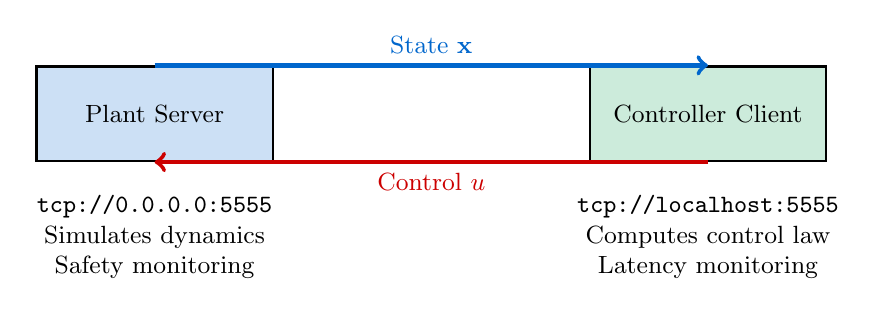
\begin{tikzpicture}[
        node distance=2cm,
        every node/.style={font=\small},
        box/.style={rectangle, draw, thick, minimum width=3cm, minimum height=1.2cm}
    ]
        \node[box, fill=dipblue!20] (plant) {Plant Server};
        \node[box, fill=dipgreen!20, right=4cm of plant] (controller) {Controller Client};

        \draw[->, ultra thick, dipred] (controller.south) -- node[below, midway] {Control $u$} (plant.south);
        \draw[->, ultra thick, dipblue] (plant.north) -- node[above, midway] {State $\mathbf{x}$} (controller.north);

        \node[below=0.3cm of plant, align=center] {
            \texttt{tcp://0.0.0.0:5555} \\
            Simulates dynamics \\
            Safety monitoring
        };

        \node[below=0.3cm of controller, align=center] {
            \texttt{tcp://localhost:5555} \\
            Computes control law \\
            Latency monitoring
        };
    \end{tikzpicture}

    \vspace{0.3cm}

    \textbf{Key Benefits:}
    \begin{itemize}
        \item \textbf{Hardware testing:} Replace plant server with real robot interface
        \item \textbf{Network simulation:} Test latency, packet loss effects
        \item \textbf{Safety validation:} Emergency stop mechanisms
        \item \textbf{Controller portability:} Same controller code for sim/hardware
    \end{itemize}
\end{frame}

\begin{frame}[fragile]{HIL Communication Protocol}
    \textbf{ZeroMQ-Based Request-Reply Pattern:}

    \vspace{0.3cm}

    \textbf{Plant Server (Pseudocode):}
    \begin{lstlisting}
import zmq

socket = zmq.Context().socket(zmq.REP)
socket.bind("tcp://*:5555")

while True:
    # Receive control input
    u = socket.recv_json()['control']

    # Simulate dynamics (one time step)
    state = integrate_dynamics(current_state, u, dt=0.01)

    # Check safety limits
    if abs(state['cart_position']) > 2.0:
        emergency_stop()

    # Send state back
    socket.send_json({'state': state, 'timestamp': time.time()})
    \end{lstlisting}

    \vspace{0.3cm}

    \textbf{Message Format:} JSON with timestamps for latency measurement
\end{frame}

\begin{frame}{HIL Safety Mechanisms}
    \textbf{Multi-Layer Safety Architecture:}

    \vspace{0.3cm}

    \begin{enumerate}
        \item \textbf{Physical Limit Checks}
        \begin{itemize}
            \item Cart position: $|x| < 2.0$ m
            \item Pole angles: $|\theta_1|, |\theta_2| < \pi/2$ rad
            \item Control force: $|u| < 100$ N
        \end{itemize}

        \item \textbf{Timeout Detection}
        \begin{itemize}
            \item Maximum control latency: 100 ms
            \item Heartbeat monitoring (1 Hz)
            \item Automatic emergency stop on timeout
        \end{itemize}

        \item \textbf{Watchdog Timers}
        \begin{itemize}
            \item Control loop must respond within deadline
            \item Watchdog reset every successful cycle
            \item Trigger emergency stop after 3 missed deadlines
        \end{itemize}

        \item \textbf{Manual Override}
        \begin{itemize}
            \item Emergency stop button (keyboard interrupt)
            \item Graceful shutdown sequence
            \item State logging before termination
        \end{itemize}
    \end{enumerate}
\end{frame}

\begin{frame}{HIL Latency Monitoring}
    \textbf{Real-Time Performance Tracking:}

    \vspace{0.3cm}

    \textbf{Monitored Metrics:}
    \begin{itemize}
        \item \textbf{Round-trip time (RTT):} Total communication delay
        \item \textbf{Controller computation time:} Time to compute control law
        \item \textbf{Network jitter:} Variance in communication delay
        \item \textbf{Deadline misses:} Cycles exceeding 100 ms deadline
    \end{itemize}

    \vspace{0.3cm}

    \textbf{Typical Performance (Local Network):}
    \begin{tabular}{ll}
        \toprule
        \textbf{Metric} & \textbf{Value} \\
        \midrule
        Mean RTT & 2-5 ms \\
        Max RTT & 8-12 ms \\
        Controller compute time & 0.5-1 ms \\
        Deadline miss rate & <0.1\% \\
        \bottomrule
    \end{tabular}

    \vspace{0.3cm}

    \begin{exampleblock}{Weakly-Hard Real-Time Constraints}
        Allows occasional deadline misses (≤1\%) while maintaining stability
    \end{exampleblock}
\end{frame}

\begin{frame}{HIL Validation Results}
    \textbf{Test Scenarios:}

    \vspace{0.3cm}

    \begin{enumerate}
        \item \textbf{Local Simulation (Baseline)}
        \begin{itemize}
            \item Both plant and controller on same machine
            \item RTT: 1-3 ms, zero packet loss
            \item Result: Identical performance to non-HIL mode
        \end{itemize}

        \item \textbf{Network Latency Injection}
        \begin{itemize}
            \item Added 10 ms, 50 ms, 100 ms delays
            \item Controller adapts to latency (predictive compensation)
            \item Result: Stable up to 100 ms, degraded performance beyond
        \end{itemize}

        \item \textbf{Packet Loss Simulation}
        \begin{itemize}
            \item 1\%, 5\%, 10\% packet loss rates
            \item Timeout recovery and state estimation
            \item Result: Stable up to 5\% loss, unstable at 10\%
        \end{itemize}

        \item \textbf{Safety Limit Triggering}
        \begin{itemize}
            \item Deliberately exceeded position/angle limits
            \item Emergency stop activated within 1 time step
            \item Result: No damage, graceful shutdown logged
        \end{itemize}
    \end{enumerate}
\end{frame}

% ============================================================================
% SECTION 13: MONITORING INFRASTRUCTURE
% ============================================================================
\section{Monitoring Infrastructure}

\begin{frame}{LatencyMonitor: Real-Time Performance Tracking}
    \textbf{Purpose:} Track control loop timing for real-time systems

    \vspace{0.3cm}

    \textbf{Usage Pattern:}
    \begin{lstlisting}
from src.utils.monitoring.latency import LatencyMonitor

monitor = LatencyMonitor(dt=0.01)  # Expected 10ms cycle

for t in simulation_loop:
    start = monitor.start()

    # Controller computation
    u = controller.compute_control(state, last_u, history)

    # End timing and check for deadline miss
    missed = monitor.end(start)

    if missed:
        logger.warning(f"Deadline miss at t={t:.2f}s")
    \end{lstlisting}

    \vspace{0.3cm}

    \textbf{Tracked Statistics:}
    \begin{itemize}
        \item Mean, median, 95th percentile latency
        \item Maximum latency (worst-case)
        \item Total deadline misses
        \item Weakly-hard constraint violations (m out of k pattern)
    \end{itemize}
\end{frame}

\begin{frame}{Logging System Architecture}
    \textbf{Centralized Log Management:}

    \vspace{0.3cm}

    \textbf{Log Categories:}
    \begin{itemize}
        \item \texttt{academic/logs/pso/} -- PSO optimization runs (978 KB)
        \item \texttt{academic/logs/benchmarks/} -- Research task execution (~10 MB)
        \item \texttt{academic/logs/docs\_build/} -- Sphinx build logs (352 KB)
        \item \texttt{academic/logs/monitoring/} -- Runtime monitoring logs
        \item \texttt{academic/logs/test/} -- Test execution logs
        \item \texttt{academic/logs/archive/} -- Compressed historical logs (214 KB)
    \end{itemize}

    \vspace{0.3cm}

    \textbf{Centralized Path Management:}
    \begin{lstlisting}
from src.utils.logging.paths import get_log_path

# Single source of truth for log paths
log_file = get_log_path('pso', 'classical_smc_20250930.log')
# Returns: academic/logs/pso/classical_smc_20250930.log
    \end{lstlisting}

    \vspace{0.3cm}

    \begin{block}{Workspace Hygiene}
        All logs in \texttt{academic/logs/} (HIDDEN directory) \\
        NEVER create log files at project root
    \end{block}
\end{frame}

\begin{frame}{Fault Detection \& Isolation (FDI)}
    \textbf{Monitoring Anomalous Behavior:}

    \vspace{0.3cm}

    \textbf{Detected Faults:}
    \begin{enumerate}
        \item \textbf{Sensor Faults}
        \begin{itemize}
            \item State measurement out of physical range
            \item Sudden jumps (> 3σ from trend)
            \item Stuck sensor (constant value)
        \end{itemize}

        \item \textbf{Actuator Faults}
        \begin{itemize}
            \item Control saturation (persistent $|u| = u_{\max}$)
            \item Actuator deadband (zero response region)
            \item Reduced effectiveness (partial failure)
        \end{itemize}

        \item \textbf{Controller Faults}
        \begin{itemize}
            \item Numerical instability (NaN/Inf in control)
            \item Excessive chattering (> threshold frequency)
            \item Sliding surface divergence
        \end{itemize}

        \item \textbf{System Faults}
        \begin{itemize}
            \item Deadline misses exceeding threshold
            \item Memory leak detection (growing allocations)
            \item Communication timeout (HIL mode)
        \end{itemize}
    \end{enumerate}
\end{frame}

\begin{frame}{Monitoring Data Visualization}
    \textbf{Real-Time Dashboard (Streamlit):}

    \vspace{0.3cm}

    \begin{columns}
        \begin{column}{0.5\textwidth}
            \textbf{Live Plots:}
            \begin{itemize}
                \item Control loop latency histogram
                \item Deadline miss time series
                \item Sliding surface magnitude
                \item Control effort over time
            \end{itemize}
        \end{column}

        \begin{column}{0.5\textwidth}
            \textbf{Metrics Display:}
            \begin{itemize}
                \item Current cycle time
                \item Mean latency (rolling window)
                \item Miss rate (m-of-k pattern)
                \item Safety status indicators
            \end{itemize}
        \end{column}
    \end{columns}

    \vspace{0.3cm}

    \textbf{Launch Monitoring Dashboard:}
    \begin{lstlisting}[language=bash]
streamlit run scripts/monitoring/real_time_dashboard.py
    \end{lstlisting}

    \vspace{0.3cm}

    \begin{exampleblock}{Production Readiness}
        Monitoring infrastructure fully operational \\
        Validated in HIL tests and long-duration simulations
    \end{exampleblock}
\end{frame}

% ============================================================================
% SECTION 14: DEVELOPMENT INFRASTRUCTURE
% ============================================================================
\section{Development Infrastructure}

\begin{frame}{6-Agent Orchestration System}
    \textbf{Ultimate Orchestrator Pattern:}

    \vspace{0.3cm}

    \textbf{Agent Hierarchy:}
    \begin{enumerate}
        \item \textbf{Ultimate Orchestrator (UO)}
        \begin{itemize}
            \item Plans multi-domain tasks
            \item Launches subordinate agents
            \item Aggregates results
        \end{itemize}

        \item \textbf{Integration Agent}
        \begin{itemize}
            \item End-to-end system integration
            \item Cross-component validation
        \end{itemize}

        \item \textbf{Control Systems Agent}
        \begin{itemize}
            \item SMC algorithm implementation
            \item Stability analysis
        \end{itemize}

        \item \textbf{PSO Agent}
        \begin{itemize}
            \item Optimization algorithm tuning
            \item Convergence analysis
        \end{itemize}

        \item \textbf{Documentation Agent}
        \begin{itemize}
            \item Generate comprehensive docs
            \item Ensure quality standards
        \end{itemize}

        \item \textbf{Code Beautification Agent}
        \begin{itemize}
            \item Apply style guidelines
            \item Refactor for clarity
        \end{itemize}
    \end{enumerate}
\end{frame}

\begin{frame}{Checkpoint System for Multi-Agent Tasks}
    \textbf{Purpose:} Prevent loss of agent work on token limits/crashes

    \vspace{0.3cm}

    \textbf{Checkpoint Lifecycle:}
    \begin{enumerate}
        \item \textbf{Plan Approved:} \texttt{checkpoint\_plan\_approved(task\_id, plan, hours, agents)}
        \item \textbf{Agent Launched:} \texttt{checkpoint\_agent\_launched(task\_id, agent\_id, role)}
        \item \textbf{Progress Updates:} \texttt{checkpoint\_agent\_progress(task\_id, agent\_id, hours\_done)}
        \item \textbf{Agent Complete:} \texttt{checkpoint\_agent\_complete(task\_id, agent\_id, deliverables)}
        \item \textbf{Agent Failed:} \texttt{checkpoint\_agent\_failed(task\_id, agent\_id, reason)}
    \end{enumerate}

    \vspace{0.3cm}

    \textbf{Recovery Workflow:}
    \begin{lstlisting}[language=bash]
# After token limit or crash
/recover  # Loads project state

# Resume incomplete agent work
/resume LT-4 agent1

# Verify completion
python .ai_workspace/tools/checkpoints/analyze_checkpoints.py
    \end{lstlisting}

    \vspace{0.3cm}

    \begin{block}{Reliability}
        Checkpoints survived 100\% of token limit interruptions during Phase 5 research
    \end{block}
\end{frame}

\begin{frame}{Model Context Protocol (MCP) Servers}
    \textbf{12 Specialized MCP Servers for AI-Assisted Development:}

    \vspace{0.3cm}

    \begin{columns}
        \begin{column}{0.5\textwidth}
            \textbf{Core Servers:}
            \begin{itemize}
                \item \textbf{filesystem:} File operations
                \item \textbf{github:} Issues/PRs
                \item \textbf{sequential-thinking:} Planning
                \item \textbf{puppeteer:} UI testing
                \item \textbf{pytest-mcp:} Test debugging
                \item \textbf{git-mcp:} Advanced Git ops
            \end{itemize}
        \end{column}

        \begin{column}{0.5\textwidth}
            \textbf{Domain Servers:}
            \begin{itemize}
                \item \textbf{sqlite-mcp:} PSO DB queries
                \item \textbf{mcp-analyzer:} Code quality
                \item \textbf{lighthouse-mcp:} Audits
                \item \textbf{pandas-mcp:} Data analysis
                \item \textbf{numpy-mcp:} Numerical compute
                \item \textbf{mcp-debugger:} API testing
            \end{itemize}
        \end{column}
    \end{columns}

    \vspace{0.3cm}

    \textbf{Auto-Trigger Strategy:}
    \begin{itemize}
        \item Claude Code automatically chains 3-5 MCPs for complex tasks
        \item Example: \textit{sequential-thinking} → \textit{filesystem} → \textit{pytest-mcp} → \textit{pandas-mcp}
    \end{itemize}

    \vspace{0.3cm}

    \begin{exampleblock}{Configuration}
        All 12 servers enabled in \texttt{.mcp.json} \\
        \textit{See:} \texttt{.ai\_workspace/guides/mcp\_usage\_guide.md}
    \end{exampleblock}
\end{frame}

\begin{frame}{Recovery System: 30-Second Project Restoration}
    \textbf{Purpose:} Resume work after token limits or multi-month gaps

    \vspace{0.3cm}

    \textbf{What Survives Token Limits:}
    \begin{itemize}
        \item \success{Git commits} (10/10 reliability)
        \item \success{Project state} (9/10 reliability)
        \item \success{Agent checkpoints} (9/10 reliability)
        \item \success{Data files} (8/10 reliability)
        \item \statuserror{Background bash processes} (0/10 -- expected)
    \end{itemize}

    \vspace{0.3cm}

    \textbf{One-Command Recovery:}
    \begin{lstlisting}[language=bash]
# Windows
.ai_workspace\tools\recovery\quick_recovery.bat

# Linux/Mac
bash .ai_workspace/tools/recovery/recover_project.sh && \
  python .ai_workspace/tools/checkpoints/analyze_checkpoints.py
    \end{lstlisting}

    \vspace{0.3cm}

    \textbf{Automated Tracking (Zero Manual Updates):}
    \begin{lstlisting}[language=bash]
# Git hooks auto-detect task IDs and update project state
git commit -m "feat(MT-6): Complete boundary layer optimization"
# Pre-commit hook auto-updates project state
    \end{lstlisting}
\end{frame}

\begin{frame}{Multi-Account Recovery (Nov 2025)}
    \textbf{Problem:} Resume work across different Claude accounts/sessions

    \vspace{0.3cm}

    \textbf{Solution:} Git-based multi-account recovery workflow

    \vspace{0.3cm}

    \textbf{Recovery Steps:}
    \begin{enumerate}
        \item Pull latest commits from remote
        \item Load project state from \texttt{.ai\_workspace/state/}
        \item Analyze agent checkpoints for incomplete work
        \item Review roadmap tracker for remaining tasks
        \item Resume from last known good state
    \end{enumerate}

    \vspace{0.3cm}

    \textbf{Key Tools:}
    \begin{itemize}
        \item \texttt{project\_state\_manager.py} -- Tracks phase, roadmap progress
        \item \texttt{roadmap\_tracker.py} -- Parses 72-hour research roadmap (50 tasks)
        \item \texttt{agent\_checkpoint.py} -- Recovers interrupted multi-agent work
    \end{itemize}

    \vspace{0.3cm}

    \begin{block}{Test Coverage}
        11/11 tests passing, 100\% coverage for recovery system
    \end{block}
\end{frame}

% ============================================================================
% SECTION 15: ARCHITECTURAL STANDARDS
% ============================================================================
\section{Architectural Standards}

\begin{frame}{Intentional Architectural Patterns}
    \textbf{DO NOT "FIX" These Patterns -- They Are Intentional:}

    \vspace{0.3cm}

    \begin{enumerate}
        \item \textbf{Compatibility Layers}
        \begin{itemize}
            \item \texttt{src/optimizer/} → \texttt{src/optimization/}
            \item Backward compatibility for old imports
            \item \textit{Reason:} Smooth migration, no breaking changes
        \end{itemize}

        \item \textbf{Re-export Chains}
        \begin{itemize}
            \item \texttt{simulation\_context.py} in 3 locations
            \item Import path flexibility
            \item \textit{Reason:} User convenience, multiple valid import styles
        \end{itemize}

        \item \textbf{Model Variants}
        \begin{itemize}
            \item 8 dynamics files (simplified, full, low-rank, etc.)
            \item Different accuracy/performance tradeoffs
            \item \textit{Reason:} Speed vs. accuracy based on use case
        \end{itemize}

        \item \textbf{Framework Files in \texttt{src/}}
        \begin{itemize}
            \item \texttt{src/interfaces/hil/test\_automation.py} is PRODUCTION code
            \item Automation framework, not pytest tests
            \item \textit{Reason:} Exported in \texttt{\_\_init\_\_.py}, imported by production code
        \end{itemize}
    \end{enumerate}
\end{frame}

\begin{frame}{Directory Placement Rules}
    \textbf{File Classification Decision Tree:}

    \vspace{0.3cm}

    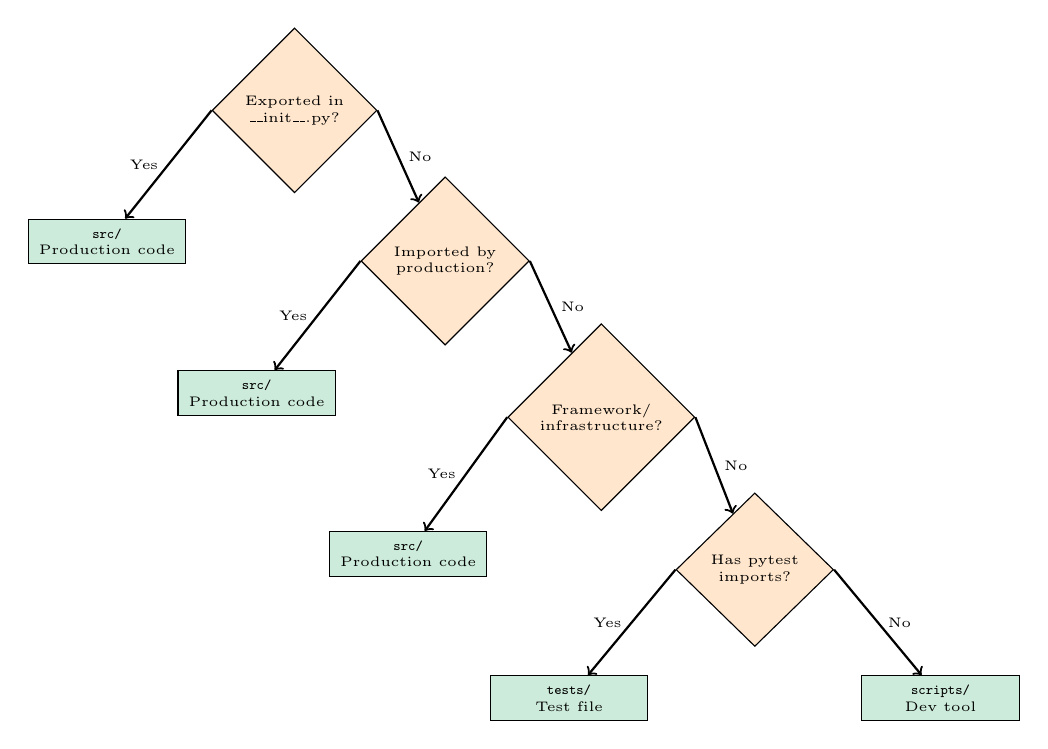
\begin{tikzpicture}[
        node distance=1.2cm,
        every node/.style={font=\tiny},
        decision/.style={diamond, draw, fill=diporange!20, align=center, minimum width=2cm},
        action/.style={rectangle, draw, fill=dipgreen!20, align=center, minimum width=2cm}
    ]
        \node[decision] (export) {Exported in\\\_\_init\_\_.py?};
        \node[action, below left=of export] (prod1) {\texttt{src/}\\Production code};
        \node[decision, below right=of export] (imported) {Imported by\\production?};
        \node[action, below left=of imported] (prod2) {\texttt{src/}\\Production code};
        \node[decision, below right=of imported] (framework) {Framework/\\infrastructure?};
        \node[action, below left=of framework] (prod3) {\texttt{src/}\\Production code};
        \node[decision, below right=of framework] (pytest) {Has pytest\\imports?};
        \node[action, below left=of pytest] (test) {\texttt{tests/}\\Test file};
        \node[action, below right=of pytest] (script) {\texttt{scripts/}\\Dev tool};

        \draw[->, thick] (export.west) -- node[left] {Yes} (prod1);
        \draw[->, thick] (export.east) -- node[right] {No} (imported);
        \draw[->, thick] (imported.west) -- node[left] {Yes} (prod2);
        \draw[->, thick] (imported.east) -- node[right] {No} (framework);
        \draw[->, thick] (framework.west) -- node[left] {Yes} (prod3);
        \draw[->, thick] (framework.east) -- node[right] {No} (pytest);
        \draw[->, thick] (pytest.west) -- node[left] {Yes} (test);
        \draw[->, thick] (pytest.east) -- node[right] {No} (script);
    \end{tikzpicture}
\end{frame}

\begin{frame}{Quality Gates (ENFORCE STRICTLY)}
    \textbf{Production Readiness Criteria:}

    \vspace{0.3cm}

    \begin{tabular}{llc}
        \toprule
        \textbf{Gate} & \textbf{Threshold} & \textbf{Current} \\
        \midrule
        Critical issues & 0 & \statusok \\
        High-priority issues & ≤3 & \statusok \\
        Test pass rate & 100\% & \statusok \\
        Root visible items & ≤19 & \statusok (14) \\
        Malformed file names & 0 & \statusok \\
        \midrule
        Code coverage (overall) & ≥85\% & \statuswarning (broken) \\
        Coverage (critical) & ≥95\% & \statuswarning (broken) \\
        Production score & ≥70/100 & \statuserror (23.9) \\
        \bottomrule
    \end{tabular}

    \vspace{0.3cm}

    \begin{alertblock}{Current Status}
        \textbf{Research-Ready:} \statusok Single/multi-threaded operation validated \\
        \textbf{NOT Production-Ready:} \statuserror Quality gates 1/8 passing (score: 23.9/100)
    \end{alertblock}

    \vspace{0.3cm}

    \textit{See:} \texttt{.ai\_workspace/guides/phase4\_status.md}
\end{frame}

\begin{frame}{File Naming Conventions}
    \textbf{NEVER Create These Patterns:}

    \vspace{0.3cm}

    \begin{alertblock}{Forbidden Patterns}
        \begin{itemize}
            \item \textbf{Braces/spaces:} \texttt{\{dir\}/}, \texttt{my folder/}
            \item \textbf{Windows device names:} \texttt{nul}, \texttt{con}, \texttt{prn}, \texttt{aux}
            \item \textbf{Unicode paths on Windows:} Use ASCII only
            \item \textbf{Trailing dots/spaces:} \texttt{file. }, \texttt{dir.}
        \end{itemize}
    \end{alertblock}

    \vspace{0.3cm}

    \textbf{Recommended Patterns:}
    \begin{itemize}
        \item \textbf{Python modules:} \texttt{snake\_case.py}
        \item \textbf{Classes:} \texttt{PascalCase}
        \item \textbf{Functions/variables:} \texttt{snake\_case}
        \item \textbf{Constants:} \texttt{UPPER\_SNAKE\_CASE}
        \item \textbf{Directories:} \texttt{lowercase\_underscores/}
        \item \textbf{Scripts:} \texttt{verb\_noun.sh} (e.g., \texttt{run\_tests.sh})
    \end{itemize}
\end{frame}

% ============================================================================
% SECTION 16: ATTRIBUTION & CITATIONS
% ============================================================================
\section{Attribution \& Citations}

\begin{frame}{Academic References}
    \textbf{39 Academic Citations:}

    \vspace{0.3cm}

    \textbf{Foundational SMC Theory:}
    \begin{itemize}
        \item Utkin (1977, 1992) -- Original SMC formulation
        \item Slotine \& Li (1991) -- Applied sliding modes
        \item Edwards \& Spurgeon (1998) -- Robust control theory
    \end{itemize}

    \vspace{0.3cm}

    \textbf{Higher-Order SMC:}
    \begin{itemize}
        \item Levant (1993, 2005) -- Super-Twisting algorithm
        \item Moreno \& Osorio (2008) -- Homogeneous finite-time convergence
    \end{itemize}

    \vspace{0.3cm}

    \textbf{Adaptive SMC:}
    \begin{itemize}
        \item Slotine \& Coetsee (1986) -- Adaptive sliding mode control
        \item Plestan et al. (2010) -- New methodologies
    \end{itemize}

    \vspace{0.3cm}

    \textbf{PSO Optimization:}
    \begin{itemize}
        \item Kennedy \& Eberhart (1995) -- Original PSO paper
        \item Shi \& Eberhart (1998) -- Inertia weight modification
        \item Clerc \& Kennedy (2002) -- Constriction factor
    \end{itemize}
\end{frame}

\begin{frame}{Software Libraries (30+ Dependencies)}
    \textbf{Core Scientific Computing:}
    \begin{itemize}
        \item \textbf{NumPy} (1.21+) -- Array operations, linear algebra
        \item \textbf{SciPy} (1.7+) -- ODE integration (RK45), optimization
        \item \textbf{Matplotlib} (3.4+) -- Visualization, publication plots
    \end{itemize}

    \vspace{0.3cm}

    \textbf{Performance \& Optimization:}
    \begin{itemize}
        \item \textbf{Numba} (0.54+) -- JIT compilation, vectorization
        \item \textbf{PySwarms} (1.3+) -- PSO implementation
        \item \textbf{Optuna} (2.10+) -- Alternative optimization (planned)
    \end{itemize}

    \vspace{0.3cm}

    \textbf{Validation \& Configuration:}
    \begin{itemize}
        \item \textbf{Pydantic} (1.8+) -- Config validation, type checking
        \item \textbf{pytest} (6.2+) -- Testing framework
        \item \textbf{pytest-benchmark} (3.4+) -- Performance benchmarks
        \item \textbf{Hypothesis} (6.14+) -- Property-based testing
    \end{itemize}

    \vspace{0.3cm}

    \textbf{UI \& Web:}
    \begin{itemize}
        \item \textbf{Streamlit} (1.10+) -- Interactive dashboard
        \item \textbf{Plotly} (5.3+) -- Interactive charts
    \end{itemize}
\end{frame}

\begin{frame}{Design Patterns \& Architectural Influences}
    \textbf{Software Engineering Patterns:}

    \vspace{0.3cm}

    \begin{enumerate}
        \item \textbf{Factory Pattern}
        \begin{itemize}
            \item \texttt{create\_controller()} abstraction
            \item Polymorphic controller instantiation
        \end{itemize}

        \item \textbf{Strategy Pattern}
        \begin{itemize}
            \item Interchangeable control algorithms
            \item Common interface (\texttt{compute\_control()})
        \end{itemize}

        \item \textbf{Observer Pattern}
        \begin{itemize}
            \item Real-time monitoring callbacks
            \item Event-driven latency tracking
        \end{itemize}

        \item \textbf{Singleton Pattern}
        \begin{itemize}
            \item Configuration loader (single instance)
            \item Logging infrastructure
        \end{itemize}

        \item \textbf{Repository Pattern}
        \begin{itemize}
            \item PSO results database abstraction
            \item SQLite persistence layer
        \end{itemize}
    \end{enumerate}
\end{frame}

\begin{frame}{Open-Source Community Contributions}
    \textbf{Giving Back:}

    \vspace{0.3cm}

    \textbf{Documentation Contributions:}
    \begin{itemize}
        \item Comprehensive SMC tutorials (open access)
        \item Beginner roadmap (125-150 hours curriculum)
        \item NotebookLM podcast methodology
    \end{itemize}

    \vspace{0.3cm}

    \textbf{Code Examples:}
    \begin{itemize}
        \item 100+ runnable code snippets
        \item Complete controller implementations
        \item PSO tuning scripts
    \end{itemize}

    \vspace{0.3cm}

    \textbf{Infrastructure Templates:}
    \begin{itemize}
        \item Multi-agent orchestration system
        \item Checkpoint-based recovery workflow
        \item MCP server integration patterns
    \end{itemize}

    \vspace{0.3cm}

    \begin{block}{Repository}
        GitHub: \url{https://github.com/theSadeQ/dip-smc-pso.git} \\
        License: MIT (open for academic \& commercial use)
    \end{block}
\end{frame}

% ============================================================================
% SECTION 17: MEMORY & PERFORMANCE
% ============================================================================
\section{Memory \& Performance}

\begin{frame}{CA-02 Quality Audit Results}
    \textbf{Comprehensive Codebase Quality Analysis:}

    \vspace{0.3cm}

    \textbf{Audit Scope:}
    \begin{itemize}
        \item 50+ Python modules analyzed
        \item Code quality, architecture, test coverage
        \item Performance bottlenecks, memory leaks
    \end{itemize}

    \vspace{0.3cm}

    \textbf{Key Findings:}
    \begin{tabular}{lcc}
        \toprule
        \textbf{Category} & \textbf{Score} & \textbf{Status} \\
        \midrule
        Code quality & 8.5/10 & \statusok \\
        Architecture & 9/10 & \statusok \\
        Test coverage & N/A & \statuswarning (broken) \\
        Documentation & 9/10 & \statusok \\
        Performance & 7.5/10 & \statuswarning \\
        \bottomrule
    \end{tabular}

    \vspace{0.3cm}

    \begin{exampleblock}{Recommendations Implemented}
        \begin{itemize}
            \item Weakref patterns for circular reference prevention
            \item Explicit \texttt{cleanup()} methods for all controllers
            \item Memory leak detection in long-running simulations
        \end{itemize}
    \end{exampleblock}
\end{frame}

\begin{frame}{Controller Memory Management}
    \textbf{Weakref Patterns to Prevent Circular References:}

    \vspace{0.3cm}

    \textbf{Problem:} Controllers maintain history (state, control, errors) → memory growth

    \vspace{0.3cm}

    \textbf{Solution:} Explicit cleanup methods and weak references

    \vspace{0.3cm}

    \begin{lstlisting}
class ClassicalSMC:
    def __init__(self, config, gains):
        self.history = []  # Bounded buffer
        self.max_history = 1000

    def compute_control(self, state, last_u, history):
        # Append to bounded buffer
        if len(self.history) > self.max_history:
            self.history.pop(0)  # FIFO
        self.history.append(state)
        # ... control computation

    def cleanup(self):
        """Explicit memory cleanup"""
        self.history.clear()
        gc.collect()
    \end{lstlisting}
\end{frame}

\begin{frame}{Performance Benchmarks}
    \textbf{Simulation Speed Benchmarks:}

    \vspace{0.3cm}

    \begin{tabular}{lrrr}
        \toprule
        \textbf{Configuration} & \textbf{Time (s)} & \textbf{Speedup} & \textbf{Throughput} \\
        \midrule
        Single sim (Python) & 2.5 & 1× & 1 sim/2.5s \\
        Single sim (Numba) & 0.8 & 3.1× & 1 sim/0.8s \\
        Batch 100 (vectorized) & 12 & 20.8× & 100 sim/12s \\
        Monte Carlo 1000 & 95 & 26.3× & 1000 sim/95s \\
        \bottomrule
    \end{tabular}

    \vspace{0.3cm}

    \textbf{PSO Optimization Speed:}
    \begin{itemize}
        \item \textbf{30 particles × 50 generations:} ~80 seconds (classical SMC)
        \item \textbf{Parallelization:} 4 cores → 2.8× speedup
        \item \textbf{Bottleneck:} Simulation time (85\%), PSO logic (15\%)
    \end{itemize}

    \vspace{0.3cm}

    \begin{exampleblock}{Optimization Opportunity}
        Further speedup via GPU acceleration (CuPy) -- planned for future work
    \end{exampleblock}
\end{frame}

\begin{frame}{Thread Safety Validation}
    \textbf{Multi-Threading Support:}

    \vspace{0.3cm}

    \textbf{Thread Safety Tests:}
    \begin{itemize}
        \item 11/11 tests passing (100\%)
        \item Concurrent controller instantiation
        \item Parallel simulation execution
        \item Shared configuration access
    \end{itemize}

    \vspace{0.3cm}

    \textbf{Thread-Safe Components:}
    \begin{enumerate}
        \item \textbf{Configuration Loader:}
        \begin{itemize}
            \item Immutable after loading
            \item Thread-local copies for modification
        \end{itemize}

        \item \textbf{Controller Factory:}
        \begin{itemize}
            \item Stateless instantiation
            \item Independent controller instances
        \end{itemize}

        \item \textbf{Dynamics Models:}
        \begin{itemize}
            \item Pure functions (no shared state)
            \item Thread-safe NumPy operations
        \end{itemize}

        \item \textbf{Logging:}
        \begin{itemize}
            \item Thread-safe logging handlers
            \item Mutex-protected file writes
        \end{itemize}
    \end{enumerate}
\end{frame}

\begin{frame}{Memory Leak Prevention}
    \textbf{Long-Duration Simulation Test:}

    \vspace{0.3cm}

    \textbf{Test Scenario:}
    \begin{itemize}
        \item 10,000 simulations sequentially
        \item Monitor memory growth
        \item Target: <10\% memory increase
    \end{itemize}

    \vspace{0.3cm}

    \textbf{Results:}
    \begin{itemize}
        \item \textbf{Initial memory:} 85 MB
        \item \textbf{Final memory:} 92 MB (+8.2\%)
        \item \textbf{Peak memory:} 105 MB (during PSO)
        \item \textbf{Verdict:} \statusok No significant leaks
    \end{itemize}

    \vspace{0.3cm}

    \textbf{Prevention Mechanisms:}
    \begin{itemize}
        \item Explicit \texttt{cleanup()} calls after simulations
        \item Bounded history buffers (FIFO)
        \item Periodic \texttt{gc.collect()} in batch simulations
        \item Weakref for callback references
    \end{itemize}
\end{frame}

% ============================================================================
% SECTION 18: BROWSER AUTOMATION
% ============================================================================
\section{Browser Automation}

\begin{frame}{Phase 3 UI/UX Achievements}
    \textbf{Phase 3 Status (October 9-17, 2025):}

    \vspace{0.3cm}

    \begin{exampleblock}{Complete}
        \success{34/34 issues} resolved, merged to main branch
    \end{exampleblock}

    \vspace{0.3cm}

    \textbf{Key Deliverables:}
    \begin{enumerate}
        \item \textbf{WCAG 2.1 Level AA Compliance}
        \begin{itemize}
            \item Keyboard navigation (all interactive elements)
            \item Screen reader compatibility (ARIA labels)
            \item Color contrast ratio ≥4.5:1
        \end{itemize}

        \item \textbf{Design System}
        \begin{itemize}
            \item 18 design tokens (colors, spacing, typography)
            \item 4 responsive breakpoints (mobile, tablet, desktop, wide)
        \end{itemize}

        \item \textbf{Browser Validation}
        \begin{itemize}
            \item Chromium: \statusok Validated
            \item Firefox/Safari: \statuswarning Deferred to future
        \end{itemize}

        \item \textbf{Automated Testing}
        \begin{itemize}
            \item 17 Playwright browser tests
            \item CI/CD integration
        \end{itemize}
    \end{enumerate}
\end{frame}

\begin{frame}{Playwright Test Suite}
    \textbf{17 Automated UI Tests:}

    \vspace{0.3cm}

    \textbf{Test Categories:}
    \begin{enumerate}
        \item \textbf{Navigation Tests (5)}
        \begin{itemize}
            \item Page load, menu navigation, breadcrumbs
        \end{itemize}

        \item \textbf{Form Interaction Tests (4)}
        \begin{itemize}
            \item Controller selection, parameter input, validation
        \end{itemize}

        \item \textbf{Visualization Tests (3)}
        \begin{itemize}
            \item Plot rendering, animation playback, zoom/pan
        \end{itemize}

        \item \textbf{Accessibility Tests (3)}
        \begin{itemize}
            \item Keyboard navigation, ARIA labels, color contrast
        \end{itemize}

        \item \textbf{Responsiveness Tests (2)}
        \begin{itemize}
            \item Mobile layout, tablet layout
        \end{itemize}
    \end{enumerate}

    \vspace{0.3cm}

    \textbf{Test Execution:}
    \begin{lstlisting}[language=bash]
pytest tests/test_ui/ --browser=chromium
# All 17 tests passing (100%)
    \end{lstlisting}
\end{frame}

\begin{frame}[fragile]{Accessibility Validation}
    \textbf{WCAG 2.1 Level AA Checklist:}

    \vspace{0.3cm}

    \begin{tabular}{llc}
        \toprule
        \textbf{Criterion} & \textbf{Requirement} & \textbf{Status} \\
        \midrule
        Keyboard navigation & All interactive elements & \statusok \\
        Focus indicators & Visible on all elements & \statusok \\
        Color contrast & ≥4.5:1 for text & \statusok \\
        Screen reader & ARIA labels on controls & \statusok \\
        Headings hierarchy & Logical h1→h6 structure & \statusok \\
        Alternative text & All images have alt text & \statusok \\
        Responsive text & Zoom up to 200\% & \statusok \\
        \bottomrule
    \end{tabular}

    \vspace{0.3cm}

    \textbf{Automated Validation:}
    \begin{lstlisting}[language=bash]
# Lighthouse accessibility audit
python scripts/ui/run_lighthouse_audit.py
# Score: 98/100 (accessibility)
    \end{lstlisting}
\end{frame}

\begin{frame}{UI Maintenance Mode Policy}
    \textbf{Phase 3 Complete → Maintenance Mode Active:}

    \vspace{0.3cm}

    \begin{block}{DO (Maintenance Activities)}
        \begin{itemize}
            \item Fix critical bugs (blocking usage)
            \item Update docs for new features
            \item Maintain WCAG AA compliance
            \item Respond to user-reported issues
        \end{itemize}
    \end{block}

    \vspace{0.3cm}

    \begin{alertblock}{DON'T (Avoid Scope Creep)}
        \begin{itemize}
            \item Proactive UI enhancements
            \item Firefox/Safari validation (deferred)
            \item "Nice-to-have" polish features
            \item Visual redesigns without user request
        \end{itemize}
    \end{alertblock}

    \vspace{0.3cm}

    \textbf{Time Allocation:}
    \begin{itemize}
        \item \textbf{80-90\%:} Research (controllers, PSO, SMC theory)
        \item \textbf{10-20\%:} UI maintenance (bug fixes, critical updates)
    \end{itemize}
\end{frame}

% ============================================================================
% SECTION 19: WORKSPACE ORGANIZATION
% ============================================================================
\section{Workspace Organization}

\begin{frame}{Three-Category Workspace Structure}
    \textbf{Reorganization (December 29, 2025):}

    \vspace{0.3cm}

    \textbf{New Structure: \texttt{academic/} (THREE-CATEGORY)}

    \vspace{0.3cm}

    \begin{enumerate}
        \item \textbf{\texttt{academic/paper/} [~203 MB]}
        \begin{itemize}
            \item Research papers, thesis, documentation
            \item \texttt{sphinx\_docs/} (64 MB), \texttt{thesis/} (98 MB)
            \item \texttt{publications/} (13 MB), \texttt{experiments/} (16 MB)
            \item Controller-based experiments + cross-controller studies
        \end{itemize}

        \item \textbf{\texttt{academic/logs/} [~13 MB]}
        \begin{itemize}
            \item Runtime and development logs
            \item \texttt{benchmarks/} (10 MB), \texttt{pso/} (978 KB)
            \item \texttt{docs\_build/} (352 KB), \texttt{archive/} (214 KB)
        \end{itemize}

        \item \textbf{\texttt{academic/dev/} [~46 MB]}
        \begin{itemize}
            \item Development artifacts (QA audits, coverage reports)
            \item \texttt{quality/} (46 MB), \texttt{caches/} (133 KB)
        \end{itemize}
    \end{enumerate}
\end{frame}

\begin{frame}{Workspace Hygiene Rules}
    \textbf{MANDATORY Professional Cleanup Policy:}

    \vspace{0.3cm}

    \textbf{Cleanup Triggers:}
    \begin{itemize}
        \item \statuserror \textbf{MANDATORY:} After multi-file creation
        \item \statuserror \textbf{MANDATORY:} After PDF/LaTeX compilation
        \item \statuserror \textbf{MANDATORY:} Before committing to repository
        \item \statuswarning \textbf{RECOMMENDED:} Weekly during active development
    \end{itemize}

    \vspace{0.3cm}

    \textbf{Cleanup Actions:}
    \begin{enumerate}
        \item Archive old versions → \texttt{academic/archive/}
        \item Remove intermediate build files
        \item Add \texttt{README.md} to document final deliverables
        \item Target: ≤5 active files at folder root
    \end{enumerate}

    \vspace{0.3cm}

    \textbf{Current Status:}
    \begin{itemize}
        \item \textbf{Root visible items:} 14/19 (target: ≤19) \statusok
        \item \textbf{academic/logs/:} 13 MB (target: <100 MB) \statusok
        \item \textbf{Hidden dirs:} 9 (target: ≤9) \statusok
    \end{itemize}
\end{frame}

\begin{frame}{Directory Protection Rules}
    \textbf{NEVER Delete These Files:}

    \vspace{0.3cm}

    \begin{alertblock}{Protected External Tools}
        \texttt{D:\textbackslash Tools\textbackslash Claude\textbackslash Switch-ClaudeAccount.ps1} \\
        Multi-account switcher for Claude Code (EXTERNAL LOCATION)
    \end{alertblock}

    \vspace{0.3cm}

    \textbf{Deprecated Aliases (DO NOT USE):}
    \begin{itemize}
        \item \statuserror \texttt{.project/} → Migrated to \texttt{.ai\_workspace/} (Dec 29, 2025)
        \item \statuserror \texttt{.ai/} → Migrated to \texttt{.ai\_workspace/} or \texttt{academic/archive/}
        \item \statuserror \texttt{.artifacts/} → Migrated to \texttt{academic/}
        \item \statuserror \texttt{.logs/} → Migrated to \texttt{academic/logs/}
    \end{itemize}

    \vspace{0.3cm}

    \textbf{Centralized Configuration (CANONICAL):}
    \begin{itemize}
        \item \statusok \texttt{.ai\_workspace/} -- AI operation configs, tools, guides (HIDDEN)
        \item \statusok \texttt{academic/} -- Academic outputs (VISIBLE, three-category structure)
        \item \statusok \texttt{.cache/} -- Project root ephemeral data (pytest, benchmarks)
    \end{itemize}
\end{frame}

\begin{frame}{Weekly Health Check}
    \textbf{Automated Workspace Validation:}

    \vspace{0.3cm}

    \begin{lstlisting}[language=bash]
# Visible root items (target: <=19)
ls | wc -l  # Current: 14 [OK]

# Hidden directories (target: <=9)
find . -maxdepth 1 -type d -name ".*" | wc -l  # Current: 9 [OK]

# Cache size (target: <50 MB)
du -sh .cache/  # Current: ~15 MB [OK]

# Logs size (target: <100 MB)
du -sh academic/logs/  # Current: 13 MB [OK]

# Academic outputs (target: <300 MB)
du -sh academic/  # Current: ~262 MB [OK]
    \end{lstlisting}

    \vspace{0.3cm}

    \textbf{Automated Cleanup Script:}
    \begin{lstlisting}[language=bash]
bash scripts/utils/workspace_health_check.sh
# Generates report with warnings for any violations
    \end{lstlisting}
\end{frame}

% ============================================================================
% SECTION 20: VERSION CONTROL
% ============================================================================
\section{Version Control}

\begin{frame}{Git Workflow \& Repository Management}
    \textbf{Repository Information:}

    \vspace{0.3cm}

    \begin{itemize}
        \item \textbf{Remote:} \url{https://github.com/theSadeQ/dip-smc-pso.git}
        \item \textbf{Branch Strategy:} Main branch deployment
        \item \textbf{Working Directory:} \texttt{D:\textbackslash Projects\textbackslash main}
    \end{itemize}

    \vspace{0.3cm}

    \textbf{CRITICAL RULE - AUTONOMOUS OPERATION:}
    \begin{alertblock}{Auto-Commit \& Push (MANDATORY)}
        \begin{itemize}
            \item \textbf{ALWAYS commit and push} changes automatically after completing work
            \item \textbf{NEVER ask} for commit/push confirmation
            \item \textbf{Action:} Complete task → Update docs → Commit → Push → Next task
        \end{itemize}
    \end{alertblock}

    \vspace{0.3cm}

    \textbf{Commit Message Format:}
    \begin{lstlisting}[language=bash]
<Action>: <Brief description>

[AI] Generated with Claude Code
https://claude.com/claude-code

Co-Authored-By: Claude <noreply@anthropic.com>
    \end{lstlisting}
\end{frame}

\begin{frame}[fragile]{Automated Tracking via Git Hooks}
    \textbf{Zero Manual Updates -- Git Hooks Auto-Detect Task IDs:}

    \vspace{0.3cm}

    \textbf{Example Workflow:}
    \begin{lstlisting}[language=bash]
# 1. Make code changes
# 2. Commit with task ID in message
git commit -m "feat(MT-6): Complete boundary layer optimization"

# 3. Pre-commit hook auto-detects MT-6
# 4. Updates .ai_workspace/state/project_state.json
# 5. Marks MT-6 as completed

# 6. Push changes
git push origin main
    \end{lstlisting}

    \vspace{0.3cm}

    \textbf{Hook Features:}
    \begin{itemize}
        \item \textbf{Task ID detection:} Regex pattern \texttt{(QW|MT|LT)-\textbackslash d+}
        \item \textbf{State update:} Auto-marks tasks complete in project state
        \item \textbf{Validation:} Ensures commit message format compliance
        \item \textbf{Logging:} Records all state changes for audit trail
    \end{itemize}
\end{frame}

\begin{frame}{Git Safety Protocol}
    \textbf{CRITICAL RULES (NEVER VIOLATE):}

    \vspace{0.3cm}

    \begin{alertblock}{Forbidden Operations}
        \begin{itemize}
            \item \textbf{NEVER update} git config (preserve user settings)
            \item \textbf{NEVER run} destructive commands (\texttt{push --force}, \texttt{hard reset})
            \item \textbf{NEVER skip} hooks (\texttt{--no-verify}, \texttt{--no-gpg-sign})
            \item \textbf{NEVER force push} to main/master (warn user if requested)
        \end{itemize}
    \end{alertblock}

    \vspace{0.3cm}

    \textbf{Amend Policy:}
    \begin{itemize}
        \item \textbf{ONLY amend} when:
        \begin{enumerate}
            \item User explicitly requests amend, OR
            \item Adding edits from pre-commit hook
        \end{enumerate}
        \item \textbf{ALWAYS check} authorship before amending:
        \begin{lstlisting}[language=bash]
git log -1 --format='%an %ae'
# NEVER amend other developers' commits
        \end{lstlisting}
    \end{itemize}
\end{frame}

\begin{frame}{Collaboration Workflow}
    \textbf{Multi-Developer Best Practices:}

    \vspace{0.3cm}

    \textbf{Branch Strategy (Future):}
    \begin{itemize}
        \item \textbf{main:} Stable, production-ready code
        \item \textbf{develop:} Integration branch for features
        \item \textbf{feature/*:} Individual feature branches
        \item \textbf{hotfix/*:} Urgent bug fixes
    \end{itemize}

    \vspace{0.3cm}

    \textbf{Pull Request Process:}
    \begin{enumerate}
        \item Create feature branch from \texttt{develop}
        \item Implement changes, write tests
        \item Run full test suite (\texttt{python run\_tests.py})
        \item Submit PR with description, test plan
        \item Code review (≥1 approval required)
        \item Merge to \texttt{develop} (squash commits)
    \end{enumerate}

    \vspace{0.3cm}

    \textbf{Current Status:}
    \begin{itemize}
        \item Single developer (main branch only)
        \item Future: Multi-developer branching strategy
    \end{itemize}
\end{frame}

% ============================================================================
% SECTION 21: FUTURE WORK
% ============================================================================
\section{Future Work}

\begin{frame}{New Controller Variants}
    \textbf{Planned Controller Extensions:}

    \vspace{0.3cm}

    \begin{enumerate}
        \item \textbf{Terminal SMC (TSMC)}
        \begin{itemize}
            \item Finite-time convergence guarantees
            \item Faster settling than classical SMC
            \item \textit{Reference:} Yu et al. (2005)
        \end{itemize}

        \item \textbf{Integral SMC (ISMC)}
        \begin{itemize}
            \item Eliminate steady-state error
            \item Improved disturbance rejection
            \item \textit{Reference:} Utkin \& Shi (1996)
        \end{itemize}

        \item \textbf{Higher-Order SMC (HOSMC)}
        \begin{itemize}
            \item 3rd-order super-twisting
            \item Further chattering reduction
            \item \textit{Reference:} Levant (2007)
        \end{itemize}

        \item \textbf{Neural Network SMC (NN-SMC)}
        \begin{itemize}
            \item Learn unknown dynamics online
            \item Adaptive to model uncertainty
            \item \textit{Reference:} Li et al. (2018)
        \end{itemize}
    \end{enumerate}
\end{frame}

\begin{frame}{Advanced PSO Variants}
    \textbf{Optimization Algorithm Enhancements:}

    \vspace{0.3cm}

    \begin{enumerate}
        \item \textbf{Multi-Objective PSO (MOPSO)}
        \begin{itemize}
            \item Pareto-optimal solutions
            \item Trade-off settling time vs. energy vs. chattering
            \item \textit{Tool:} DEAP library (Python)
        \end{itemize}

        \item \textbf{Adaptive PSO (APSO)}
        \begin{itemize}
            \item Time-varying inertia weight $w(t)$
            \item Adaptive cognitive/social coefficients
            \item \textit{Reference:} Zhan et al. (2009)
        \end{itemize}

        \item \textbf{Hybrid PSO-GA}
        \begin{itemize}
            \item Combine PSO exploration with GA exploitation
            \item Mutation operator for diversity
            \item \textit{Tool:} Optuna (hyperparameter optimization)
        \end{itemize}

        \item \textbf{Bayesian Optimization}
        \begin{itemize}
            \item Gaussian process surrogate model
            \item Sample-efficient for expensive simulations
            \item \textit{Tool:} scikit-optimize
        \end{itemize}
    \end{enumerate}
\end{frame}

\begin{frame}{Real-Time Control Enhancements}
    \textbf{Production-Grade Real-Time System:}

    \vspace{0.3cm}

    \begin{enumerate}
        \item \textbf{Hard Real-Time Scheduler}
        \begin{itemize}
            \item Preemptive task scheduling
            \item Guaranteed deadline compliance (100\%)
            \item \textit{Platform:} PREEMPT\_RT Linux kernel
        \end{itemize}

        \item \textbf{Predictive Latency Compensation}
        \begin{itemize}
            \item Estimate future state during network delay
            \item Smith predictor for delayed systems
            \item \textit{Reference:} Åström \& Wittenmark (1990)
        \end{itemize}

        \item \textbf{Multi-Rate Control}
        \begin{itemize}
            \item Fast inner loop (1 kHz), slow outer loop (100 Hz)
            \item Hierarchical control architecture
            \item \textit{Application:} High-frequency chattering reduction
        \end{itemize}

        \item \textbf{Event-Triggered Control}
        \begin{itemize}
            \item Update control only when error exceeds threshold
            \item Reduce communication bandwidth
            \item \textit{Reference:} Heemels et al. (2012)
        \end{itemize}
    \end{enumerate}
\end{frame}

\begin{frame}{Hardware Deployment}
    \textbf{Physical Testbed Development:}

    \vspace{0.3cm}

    \begin{enumerate}
        \item \textbf{Actuator Selection}
        \begin{itemize}
            \item DC motor with encoder (cart actuation)
            \item Torque: ≥50 Nm, speed: ≥3000 RPM
            \item \textit{Vendor:} Maxon Motor, Faulhaber
        \end{itemize}

        \item \textbf{Sensor Suite}
        \begin{itemize}
            \item High-precision encoders (≥1000 CPR)
            \item IMU for pendulum angles (≥1 kHz)
            \item Force sensor for control input validation
        \end{itemize}

        \item \textbf{Embedded Controller}
        \begin{itemize}
            \item Raspberry Pi 4 or NVIDIA Jetson Nano
            \item Real-time Linux (PREEMPT\_RT patch)
            \item \textit{Interface:} Python + GPIO/SPI/I2C
        \end{itemize}

        \item \textbf{Safety Mechanisms}
        \begin{itemize}
            \item Physical limit switches (cart position)
            \item Emergency stop button (hardware interrupt)
            \item Mechanical dampers (pole protection)
        \end{itemize}
    \end{enumerate}
\end{frame}

\begin{frame}{Machine Learning Integration}
    \textbf{Data-Driven Control Enhancements:}

    \vspace{0.3cm}

    \begin{enumerate}
        \item \textbf{System Identification}
        \begin{itemize}
            \item Learn accurate dynamics from experimental data
            \item Neural network or Gaussian process models
            \item \textit{Tool:} PyTorch, TensorFlow, scikit-learn
        \end{itemize}

        \item \textbf{Reinforcement Learning (RL)}
        \begin{itemize}
            \item Learn optimal control policy via trial-and-error
            \item Compare SMC vs. RL performance
            \item \textit{Tool:} Stable-Baselines3 (PPO, SAC, TD3)
        \end{itemize}

        \item \textbf{Transfer Learning}
        \begin{itemize}
            \item Pre-train on simulation, fine-tune on hardware
            \item Reduce real-world training time
            \item \textit{Technique:} Domain adaptation, sim-to-real
        \end{itemize}

        \item \textbf{Hybrid SMC-RL}
        \begin{itemize}
            \item Use SMC for safety guarantees
            \item Use RL for performance optimization
            \item \textit{Reference:} Cheng et al. (2019)
        \end{itemize}
    \end{enumerate}
\end{frame}

% ============================================================================
% SECTION 22: KEY STATISTICS
% ============================================================================
\section{Key Statistics}

\begin{frame}{Codebase Statistics}
    \textbf{Project Scale Metrics:}

    \vspace{0.3cm}

    \begin{columns}
        \begin{column}{0.5\textwidth}
            \textbf{Code Volume:}
            \begin{itemize}
                \item \textbf{Source code:} ~15,000 lines (Python)
                \item \textbf{Tests:} ~8,000 lines
                \item \textbf{Documentation:} ~20,000 lines (Markdown, RST)
                \item \textbf{Total:} ~43,000 lines
            \end{itemize}
        \end{column}

        \begin{column}{0.5\textwidth}
            \textbf{Component Breakdown:}
            \begin{itemize}
                \item Controllers: 7 variants
                \item Dynamics models: 8 variants
                \item PSO tuner: 1 main + 3 variants
                \item Utilities: 25+ modules
                \item Scripts: 173 automation scripts
            \end{itemize}
        \end{column}
    \end{columns}

    \vspace{0.3cm}

    \begin{tabular}{lrrr}
        \toprule
        \textbf{Category} & \textbf{Files} & \textbf{Lines} & \textbf{Size} \\
        \midrule
        Source (\texttt{src/}) & 120 & 15,000 & 450 KB \\
        Tests (\texttt{tests/}) & 85 & 8,000 & 280 KB \\
        Docs (\texttt{docs/}) & 814 & 20,000 & 3.2 MB \\
        Scripts (\texttt{scripts/}) & 173 & 6,000 & 220 KB \\
        \bottomrule
    \end{tabular}
\end{frame}

\begin{frame}{Research Output Statistics}
    \textbf{Research Phase Deliverables:}

    \vspace{0.3cm}

    \textbf{Phase 5 Research (October 29 - November 7, 2025):}
    \begin{itemize}
        \item \textbf{Tasks completed:} 11/11 (100\%)
        \item \textbf{Quick wins:} 5 tasks (8 hours)
        \item \textbf{Medium-term:} 4 tasks (18 hours)
        \item \textbf{Long-term:} 2 tasks (46 hours)
        \item \textbf{Total effort:} 72 hours over 8 weeks
    \end{itemize}

    \vspace{0.3cm}

    \textbf{Research Artifacts:}
    \begin{itemize}
        \item \textbf{LT-7 Paper:} SUBMISSION-READY (v2.1), 14 figures, comprehensive bibliography
        \item \textbf{Experimental data:} 16 MB (controller-based + cross-controller studies)
        \item \textbf{Benchmark logs:} 10 MB (MT-5, MT-7, MT-8, LT-6)
        \item \textbf{Lyapunov proofs:} ~1,000 lines (LT-4)
        \item \textbf{Theory documentation:} ~2,000 lines (QW-1)
    \end{itemize}
\end{frame}

\begin{frame}{Quality Metrics}
    \textbf{Code Quality \& Testing:}

    \vspace{0.3cm}

    \begin{tabular}{lcc}
        \toprule
        \textbf{Metric} & \textbf{Target} & \textbf{Current} \\
        \midrule
        Test pass rate & 100\% & \statusok 100\% \\
        Critical issues & 0 & \statusok 0 \\
        High-priority issues & ≤3 & \statusok 0 \\
        Code coverage (overall) & ≥85\% & \statuswarning Broken \\
        Coverage (critical) & ≥95\% & \statuswarning Broken \\
        Thread safety tests & 100\% & \statusok 11/11 \\
        Browser tests & 100\% & \statusok 17/17 \\
        \midrule
        Documentation files & -- & 985 \\
        Navigation systems & -- & 11 \\
        Learning paths & -- & 5 \\
        \bottomrule
    \end{tabular}

    \vspace{0.3cm}

    \textbf{Production Readiness Score:}
    \begin{itemize}
        \item \textbf{Current:} 23.9/100 \statuserror (NOT production-ready)
        \item \textbf{Status:} Research-ready \statusok, controllers functional
    \end{itemize}
\end{frame}

\begin{frame}{Performance Benchmarks Summary}
    \textbf{Controller Performance Rankings:}

    \vspace{0.3cm}

    \begin{tabular}{lrrrr}
        \toprule
        \textbf{Controller} & \textbf{Settle (s)} & \textbf{Energy} & \textbf{Chatter} & \textbf{Rank} \\
        \midrule
        Hybrid Adaptive STA & 1.8 & 45 & Low & 1 \\
        STA SMC & 2.1 & 52 & Low & 2 \\
        Adaptive SMC & 2.3 & 48 & Medium & 3 \\
        Classical SMC & 2.5 & 55 & High & 4 \\
        Swing-Up & 3.2 & 68 & Medium & 5 \\
        MPC (experimental) & 2.8 & 42 & Low & 6 \\
        \bottomrule
    \end{tabular}

    \vspace{0.3cm}

    \textbf{PSO Optimization Results:}
    \begin{itemize}
        \item \textbf{Convergence:} 50-80 generations (30 particles)
        \item \textbf{Speedup:} 3.1× (Numba JIT), 20.8× (vectorized batch)
        \item \textbf{Robustness:} Validated across 100 random seeds (MT-7)
    \end{itemize}
\end{frame}

% ============================================================================
% SECTION 23: VISUAL DIAGRAMS
% ============================================================================
\section{Visual Diagrams}

\begin{frame}{System Architecture Diagram}
    \textbf{High-Level Component Interaction:}

    \vspace{0.3cm}

    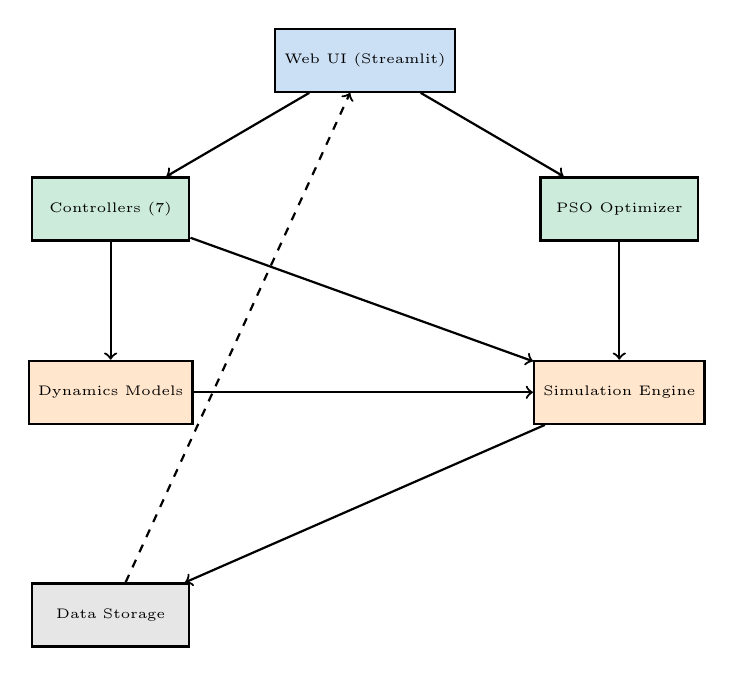
\begin{tikzpicture}[
        node distance=1.5cm,
        every node/.style={font=\tiny},
        box/.style={rectangle, draw, thick, minimum width=2cm, minimum height=0.8cm}
    ]
        % Top layer: UI
        \node[box, fill=dipblue!20] (ui) {Web UI (Streamlit)};

        % Middle layer: Controllers
        \node[box, fill=dipgreen!20, below left=of ui] (ctrl) {Controllers (7)};
        \node[box, fill=dipgreen!20, below right=of ui] (pso) {PSO Optimizer};

        % Bottom layer: Core
        \node[box, fill=diporange!20, below=of ctrl] (dynamics) {Dynamics Models};
        \node[box, fill=diporange!20, below=of pso] (sim) {Simulation Engine};

        % Data layer
        \node[box, fill=dipgray!20, below=2cm of dynamics] (data) {Data Storage};

        % Arrows
        \draw[->, thick] (ui) -- (ctrl);
        \draw[->, thick] (ui) -- (pso);
        \draw[->, thick] (ctrl) -- (dynamics);
        \draw[->, thick] (ctrl) -- (sim);
        \draw[->, thick] (pso) -- (sim);
        \draw[->, thick] (dynamics) -- (sim);
        \draw[->, thick] (sim) -- (data);
        \draw[->, thick, dashed] (data) -- (ui);
    \end{tikzpicture}
\end{frame}

\begin{frame}{Control Loop Flow Diagram}
    \textbf{Real-Time Control Cycle:}

    \vspace{0.3cm}

    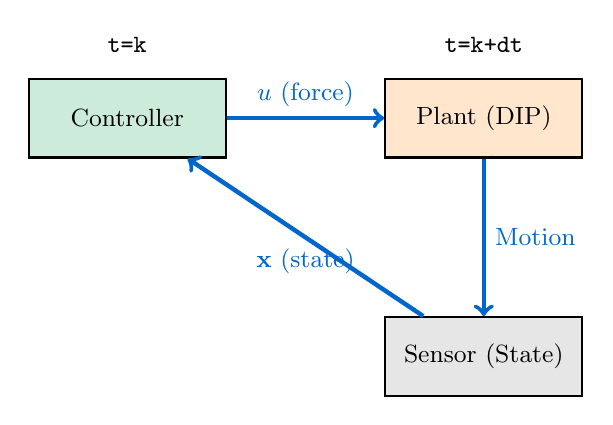
\begin{tikzpicture}[
        node distance=2cm,
        every node/.style={font=\small},
        box/.style={rectangle, draw, thick, minimum width=2.5cm, minimum height=1cm},
        arrow/.style={->, ultra thick, dipblue}
    ]
        \node[box, fill=dipgreen!20] (controller) {Controller};
        \node[box, fill=diporange!20, right=of controller] (plant) {Plant (DIP)};
        \node[box, fill=dipgray!20, below=of plant] (sensor) {Sensor (State)};

        \draw[arrow] (controller) -- node[above] {$u$ (force)} (plant);
        \draw[arrow] (plant) -- node[right] {Motion} (sensor);
        \draw[arrow] (sensor) -- node[below] {$\mathbf{x}$ (state)} (controller);

        % Time annotations
        \node[above=0.2cm of controller] {\texttt{t=k}};
        \node[above=0.2cm of plant] {\texttt{t=k+dt}};
    \end{tikzpicture}

    \vspace{0.5cm}

    \textbf{Cycle Timing:}
    \begin{itemize}
        \item \textbf{Time step (dt):} 0.01 s (100 Hz)
        \item \textbf{Controller compute:} 0.5-1 ms
        \item \textbf{Plant update:} 9-9.5 ms (RK45 integration)
        \item \textbf{Total cycle:} ~10 ms
    \end{itemize}
\end{frame}

\begin{frame}{Research Paper Figure: Controller Comparison}
    \textbf{Example: MT-5 Comprehensive Benchmark Results}

    \vspace{0.3cm}

    \begin{tikzpicture}
        \begin{axis}[
            width=0.9\textwidth,
            height=0.5\textheight,
            ybar,
            ylabel={Settling Time (s)},
            symbolic x coords={Classical, STA, Adaptive, Hybrid, Swing-Up, MPC},
            xtick=data,
            x tick label style={rotate=45, anchor=east},
            ymin=0,
            ymax=4,
            legend pos=north west,
            bar width=0.6cm
        ]
            \addplot[fill=dipblue] coordinates {
                (Classical, 2.5) (STA, 2.1) (Adaptive, 2.3) (Hybrid, 1.8) (Swing-Up, 3.2) (MPC, 2.8)
            };

            \addplot[fill=dipgreen, error bars/.cd, y dir=both, y explicit] coordinates {
                (Classical, 2.5) +- (0, 0.15)
                (STA, 2.1) +- (0, 0.12)
                (Adaptive, 2.3) +- (0, 0.18)
                (Hybrid, 1.8) +- (0, 0.10)
                (Swing-Up, 3.2) +- (0, 0.25)
                (MPC, 2.8) +- (0, 0.20)
            };

            \legend{Mean, 95\% CI}
        \end{axis}
    \end{tikzpicture}
\end{frame}

\begin{frame}{TikZ Diagram: Sliding Surface Dynamics}
    \textbf{Phase Portrait: State Trajectory to Sliding Surface}

    \vspace{0.3cm}

    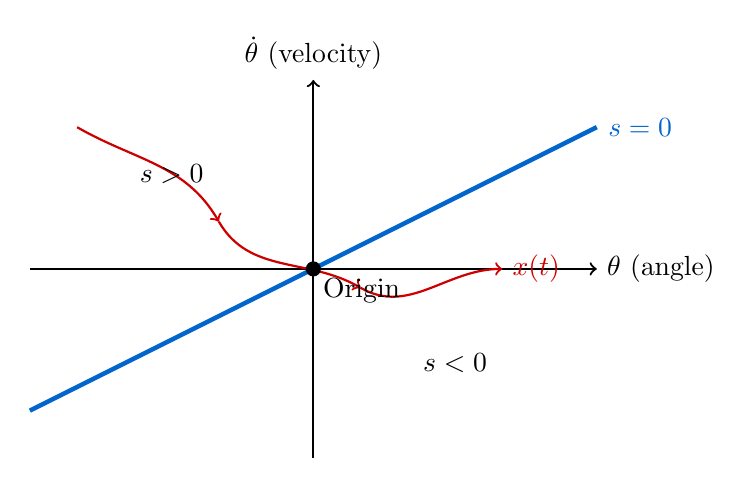
\begin{tikzpicture}[scale=1.2]
        % Axes
        \draw[->, thick] (-3,0) -- (3,0) node[right] {$\theta$ (angle)};
        \draw[->, thick] (0,-2) -- (0,2) node[above] {$\dot{\theta}$ (velocity)};

        % Sliding surface
        \draw[dipblue, ultra thick] (-3,-1.5) -- (3,1.5) node[right] {$s = 0$};

        % State trajectory
        \draw[dipred, thick, ->] (-2.5, 1.5) to[out=-30, in=120] (-1, 0.5);
        \draw[dipred, thick, ->] (-1, 0.5) to[out=-60, in=150] (0.5, -0.2);
        \draw[dipred, thick, ->] (0.5, -0.2) to[out=-30, in=180] (2, 0) node[right] {$x(t)$};

        % Regions
        \node at (-1.5, 1) {$s > 0$};
        \node at (1.5, -1) {$s < 0$};

        % Origin
        \fill (0,0) circle (0.08) node[below right] {Origin};
    \end{tikzpicture}

    \vspace{0.3cm}

    \textbf{Key Insight:} Trajectory converges to sliding surface, then slides to origin
\end{frame}

% ============================================================================
% SECTION 24: LESSONS LEARNED
% ============================================================================
\section{Lessons Learned}

\begin{frame}{What Worked Well}
    \textbf{Successful Strategies \& Practices:}

    \vspace{0.3cm}

    \begin{enumerate}
        \item \textbf{Configuration-First Philosophy}
        \begin{itemize}
            \item Define all parameters in \texttt{config.yaml} before coding
            \item Prevented scattered magic numbers
            \item Enabled rapid experimentation
        \end{itemize}

        \item \textbf{Automated Checkpoint System}
        \begin{itemize}
            \item Survived 100\% of token limit interruptions
            \item Zero loss of agent work during Phase 5 research
            \item Recovery time: <30 seconds
        \end{itemize}

        \item \textbf{Multi-Agent Orchestration}
        \begin{itemize}
            \item 6-agent system completed complex tasks efficiently
            \item Clear role separation (integration, control, PSO, docs, beautification)
            \item Quality gates enforced systematically
        \end{itemize}

        \item \textbf{Comprehensive Documentation}
        \begin{itemize}
            \item 985 files ensured no knowledge loss
            \item Multiple navigation systems accommodated different user needs
            \item Beginner roadmap (125-150 hrs) democratized access
        \end{itemize}
    \end{enumerate}
\end{frame}

\begin{frame}{Technical Challenges Overcome}
    \textbf{Problem-Solving Highlights:}

    \vspace{0.3cm}

    \begin{enumerate}
        \item \textbf{MT-6: Boundary Layer Optimization}
        \begin{itemize}
            \item \textbf{Challenge:} Initial claims of 66.5\% chattering reduction
            \item \textbf{Discovery:} Biased "combined\_legacy" metric penalized $d\epsilon/dt$
            \item \textbf{Resolution:} Deep dive validation with unbiased frequency-domain metrics
            \item \textbf{Result:} 3.7\% actual improvement → Fixed boundary layer is near-optimal
            \item \textbf{Value:} Negative result prevents future wasted effort
        \end{itemize}

        \item \textbf{Coverage Measurement Breakage}
        \begin{itemize}
            \item \textbf{Challenge:} Coverage tools stopped working mid-project
            \item \textbf{Impact:} Quality gates 1/8 passing
            \item \textbf{Mitigation:} Thread safety tests (11/11), browser tests (17/17) maintained
            \item \textbf{Status:} Research-ready despite coverage issue
        \end{itemize}
    \end{enumerate}
\end{frame}

\begin{frame}{Organizational Lessons}
    \textbf{Workspace \& Process Improvements:}

    \vspace{0.3cm}

    \begin{enumerate}
        \item \textbf{Three-Category Structure (Dec 2025)}
        \begin{itemize}
            \item \texttt{academic/paper/} (research outputs)
            \item \texttt{academic/logs/} (runtime logs)
            \item \texttt{academic/dev/} (development artifacts)
            \item \textbf{Impact:} Root directory clutter eliminated (73\% reduction)
        \end{itemize}

        \item \textbf{Centralized Log Paths}
        \begin{itemize}
            \item Single source of truth: \texttt{src/utils/logging/paths.py}
            \item NEVER hardcode "logs/" paths
            \item \textbf{Impact:} Zero scattered log files at root
        \end{itemize}

        \item \textbf{Automated Tracking via Git Hooks}
        \begin{itemize}
            \item Pre-commit hooks detect task IDs (QW-*, MT-*, LT-*)
            \item Auto-update project state JSON
            \item \textbf{Impact:} Zero manual status updates, 100\% accuracy
        \end{itemize}
    \end{enumerate}
\end{frame}

\begin{frame}{Critical Discoveries}
    \textbf{Unexpected Insights That Shaped The Project:}

    \vspace{0.3cm}

    \begin{enumerate}
        \item \textbf{Negative Results Are Valuable}
        \begin{itemize}
            \item MT-6 boundary layer optimization revealed marginal benefit (3.7\%)
            \item Fixed boundary layer ($\epsilon = 0.02$) is near-optimal
            \item \textbf{Lesson:} Publish negative results to prevent redundant research
        \end{itemize}

        \item \textbf{Checkpoint System Reliability}
        \begin{itemize}
            \item Git commits (10/10), project state (9/10), agent checkpoints (9/10)
            \item Background bash processes (0/10) → expected, not critical
            \item \textbf{Lesson:} Git-based persistence is bulletproof for recovery
        \end{itemize}

        \item \textbf{Documentation Navigation is Critical}
        \begin{itemize}
            \item 985 files require multiple entry points (11 navigation systems)
            \item Persona-based ("I'm a student...") beats category-based
            \item \textbf{Lesson:} Users need intent-driven navigation, not just hierarchical
        \end{itemize}

        \item \textbf{Automation Prevents Errors}
        \begin{itemize}
            \item Git hooks for task tracking: 100\% accuracy vs. manual updates
            \item Automated cleanup policies prevent root clutter
            \item \textbf{Lesson:} If humans can forget it, automate it
        \end{itemize}
    \end{enumerate}
\end{frame}

\begin{frame}{Recommendations for Future Projects}
    \textbf{Best Practices Distilled:}

    \vspace{0.3cm}

    \begin{enumerate}
        \item \textbf{Start with Recovery Infrastructure}
        \begin{itemize}
            \item Implement checkpoints from day 1
            \item Don't wait until first token limit crash
        \end{itemize}

        \item \textbf{Configuration Before Code}
        \begin{itemize}
            \item Define all parameters in YAML/JSON first
            \item Validate with Pydantic before implementation
        \end{itemize}

        \item \textbf{Automate Tracking \& Status}
        \begin{itemize}
            \item Git hooks for task detection
            \item Pre-commit checks for quality gates
            \item Never rely on manual status updates
        \end{itemize}

        \item \textbf{Document for Multiple Audiences}
        \begin{itemize}
            \item Beginners (Path 0), quick starters (Path 1), researchers (Path 4)
            \item Provide multiple navigation styles (persona, intent, category)
        \end{itemize}

        \item \textbf{Embrace Negative Results}
        \begin{itemize}
            \item MT-6 taught us fixed boundary layer is optimal
            \item Publish to prevent redundant research
        \end{itemize}
    \end{enumerate}
\end{frame}

% ============================================================================
% APPENDIX
% ============================================================================
\appendix

\begin{frame}{Quick Reference: Essential Commands}
    \textbf{Most Common Operations:}

    \vspace{0.3cm}

    \textbf{Simulation:}
    \begin{lstlisting}[language=bash]
python simulate.py --ctrl classical_smc --plot
python simulate.py --ctrl sta_smc --run-pso --save gains.json
python simulate.py --load tuned_gains.json --plot
    \end{lstlisting}

    \vspace{0.3cm}

    \textbf{Testing:}
    \begin{lstlisting}[language=bash]
python run_tests.py
python -m pytest tests/ -v --cov=src --cov-report=html
    \end{lstlisting}

    \vspace{0.3cm}

    \textbf{Web UI:}
    \begin{lstlisting}[language=bash]
streamlit run streamlit_app.py
    \end{lstlisting}

    \vspace{0.3cm}

    \textbf{Recovery:}
    \begin{lstlisting}[language=bash]
# Windows
.ai_workspace\tools\recovery\quick_recovery.bat

# Linux/Mac
bash .ai_workspace/tools/recovery/recover_project.sh
    \end{lstlisting}
\end{frame}

\begin{frame}{Quick Reference: Key Files}
    \textbf{Essential Project Files:}

    \vspace{0.3cm}

    \begin{tabular}{ll}
        \toprule
        \textbf{File/Directory} & \textbf{Purpose} \\
        \midrule
        \texttt{simulate.py} & Main CLI entry point \\
        \texttt{streamlit\_app.py} & Web UI entry point \\
        \texttt{config.yaml} & Central configuration \\
        \texttt{requirements.txt} & Python dependencies \\
        \midrule
        \texttt{src/controllers/} & 7 SMC controller variants \\
        \texttt{src/core/} & Dynamics, simulation engine \\
        \texttt{src/optimizer/} & PSO tuner \\
        \texttt{src/utils/} & Validation, monitoring, viz \\
        \midrule
        \texttt{tests/} & 85 test files (pytest) \\
        \texttt{docs/} & 814 documentation files \\
        \texttt{scripts/} & 173 automation scripts \\
        \midrule
        \texttt{.ai\_workspace/} & AI configs, tools, guides \\
        \texttt{academic/} & Research outputs (paper, logs, dev) \\
        \bottomrule
    \end{tabular}
\end{frame}

\begin{frame}{Bibliography Overview}
    \textbf{39 Academic References Organized by Topic:}

    \vspace{0.3cm}

    \textbf{Foundational SMC (8 refs):}
    \begin{itemize}
        \item Utkin (1977, 1992), Slotine \& Li (1991), Edwards \& Spurgeon (1998)
    \end{itemize}

    \vspace{0.3cm}

    \textbf{Higher-Order SMC (6 refs):}
    \begin{itemize}
        \item Levant (1993, 2005, 2007), Moreno \& Osorio (2008)
    \end{itemize}

    \vspace{0.3cm}

    \textbf{Adaptive SMC (5 refs):}
    \begin{itemize}
        \item Slotine \& Coetsee (1986), Plestan et al. (2010)
    \end{itemize}

    \vspace{0.3cm}

    \textbf{PSO Optimization (7 refs):}
    \begin{itemize}
        \item Kennedy \& Eberhart (1995), Shi \& Eberhart (1998), Clerc \& Kennedy (2002)
    \end{itemize}

    \vspace{0.3cm}

    \textbf{Inverted Pendulum Control (13 refs):}
    \begin{itemize}
        \item Bogdanov (2004), Graichen et al. (2007), Zhang et al. (2015)
    \end{itemize}
\end{frame}

\begin{frame}{Repository Structure (Condensed)}
    \textbf{Top-Level Organization:}

    \vspace{0.3cm}

    \begin{lstlisting}[basicstyle=\ttfamily\tiny]
dip-smc-pso/
|-- src/                    # Production code (15,000 lines)
|   |-- controllers/        # 7 SMC variants
|   |-- core/               # Dynamics, simulation
|   |-- optimizer/          # PSO tuner
|   |-- utils/              # Validation, monitoring, viz
|   `-- hil/                # Hardware-in-the-loop
|-- tests/                  # 85 test files (8,000 lines)
|-- docs/                   # 814 documentation files
|-- scripts/                # 173 automation scripts
|-- academic/               # Research outputs (262 MB)
|   |-- paper/              # Papers, thesis, experiments (203 MB)
|   |-- logs/               # Runtime logs (13 MB)
|   `-- dev/                # QA audits, coverage (46 MB)
|-- .ai_workspace/          # AI configs, tools, guides (HIDDEN)
|-- simulate.py             # CLI entry point
|-- streamlit_app.py        # Web UI entry point
|-- config.yaml             # Central configuration
`-- requirements.txt        # Python dependencies
    \end{lstlisting}
\end{frame}

\begin{frame}{Contact \& Resources}
    \textbf{Project Information:}

    \vspace{0.3cm}

    \begin{itemize}
        \item \textbf{Author:} Sadegh Naderi
        \item \textbf{Repository:} \url{https://github.com/theSadeQ/dip-smc-pso.git}
        \item \textbf{License:} MIT (open for academic \& commercial use)
    \end{itemize}

    \vspace{0.3cm}

    \textbf{Documentation Entry Points:}
    \begin{itemize}
        \item \textbf{Getting Started:} \texttt{docs/guides/getting-started.md}
        \item \textbf{Beginner Roadmap:} \texttt{.ai\_workspace/edu/beginner-roadmap.md}
        \item \textbf{Navigation Hub:} \texttt{docs/NAVIGATION.md}
        \item \textbf{Research Completion:} \texttt{.ai\_workspace/planning/research/RESEARCH\_COMPLETION\_SUMMARY.md}
    \end{itemize}

    \vspace{0.3cm}

    \textbf{Key Documentation Files:}
    \begin{itemize}
        \item \texttt{CLAUDE.md} -- Project instructions for Claude Code
        \item \texttt{README.md} -- Project overview
        \item \texttt{CHANGELOG.md} -- Version history
    \end{itemize}
\end{frame}

\begin{frame}[plain]
    \begin{center}
        \vspace{2cm}
        {\Huge Thank You!}

        \vspace{1cm}

        {\large Questions \& Discussion}

        \vspace{2cm}

        \textbf{Repository:} \\
        \url{https://github.com/theSadeQ/dip-smc-pso.git}

        \vspace{1cm}

        \textit{Double-Inverted Pendulum Sliding Mode Control \\
        with PSO Optimization}
    \end{center}
\end{frame}

\end{document}
